% Copyright (C) 2010-2012 Matthew Ruffoni
%
% This file is part of FAST.
%
% DEXA is free software: you can redistribute it and/or modify
% it under the terms of the GNU General Public License as published by
% the Free Software Foundation, either version 3 of the License, or
% (at your option) any later version.
%
% DEXA is distributed in the hope that it will be useful,
% but WITHOUT ANY WARRANTY; without even the implied warranty of
% MERCHANTABILITY or FITNESS FOR A PARTICULAR PURPOSE.  See the
% GNU General Public License for more details.
%
% You should have received a copy of the GNU General Public License
% along with DEXA.  If not, see <http://www.gnu.org/licenses/>.
%
\documentclass[a4paper,12pt]{report}
\usepackage{graphicx}
\usepackage{color}
\usepackage{enumerate}
\newcommand{\fast}{\emph{FAST} }
\newcommand{\xgremlin}{\emph{XGremlin} }
\hyphenation{FAST}
\hyphenation{XGremlin}

\definecolor{weak_found}{rgb}{0.375,0.375,0.375}
\definecolor{weak_not_found}{rgb}{0.8125,0.8125,0.8125}
\definecolor{strong_not_found}{rgb}{1,0.5625,0.5625}
\definecolor{int_not_calibrated}{rgb}{1,0.8118,0.8118}
\definecolor{int_calibrated}{rgb}{0.8118,1,0.8118}
\definecolor{attached_line_list}{rgb}{1,1,0.6863}
\definecolor{attached_std_lamp}{rgb}{0.6863,1,0.6863}
\definecolor{attached_link}{rgb}{0.6863,0.6863,1}

\title{The FTS Atomic Spectrum Tool (FAST) \\ User Manual}
\begin{document}
\maketitle 
\tableofcontents
\chapter{An Important Disclaimer}
\section{\fast development is ongoing}
\fast is still in the early stages of development. Some functionality that would be desirable for a 'final' version 1.0 is still missing, and other features present in the current version are still not fully mature. More importantly though, it is inevitable that some bugs are still present in the software, and impossible to rule out the possibility that one or more of them result in the wrong answers being given under certain conditions.

During development to date, the code has been tested with synthetic data sets as well as a number of real experimental line spectra. The results from these tests were good, and the overall program considered sufficiently stable, to warrant this release.

However, be on your guard at all times when analysing your own data. Check all the numbers given by \fast to make sure they are correct. As stated in the GNU General Public License
\begin{quote}
{\bf``This program is distributed in the hope that it will be useful,
but WITHOUT ANY WARRANTY; without even the implied warranty of
MERCHANTABILITY or FITNESS FOR A PARTICULAR PURPOSE."}
\end{quote}
You have been warned!

\section{Bug reporting}
If, in the course of using \fast, you encounter any bugs, please report them to me at m.ruffoni@imperial.ac.uk

If possible (and assuming they are not too large) include your original data files and any information you think necessary for me to reproduce the bug.

Please also get in touch if you would be interested in helping with the future development of \emph{FAST}; be it as a programmer, tester, or simply to suggest improvements.

\chapter{Installing \fast}
\section{Installing pre-compiled binaries}
Binaries are available for download from the \fast website for various (predominantly Linux-based) systems. Follow the individual system-specific instructions to install \emph{FAST}. If a binary is not available for your system, you will need to download the raw source code and compile it yourself.
\section{Installing from the raw source code}
\label{section:inst:code}
Before starting, make sure you have the following programs available:

\begin{enumerate}
\item The GNU \verb|g++| compiler. 
\item The GNU Scientific Library (\verb|gsl|). 
\item GNU \verb|make| to run the \verb|Makefile| generated by the \verb|configure| script.
\item The GTK+ library and its \verb|gtkmm| implementation.
\end{enumerate}
Assuming these are present, open a standard terminal window and enter
\begin{quote}
  user\@@host: \texttt{cd \emph{<directory where you unpacked FAST>}}\\
  user\@@host: \verb|./configure|\\
  user\@@host: \verb|make|
\end{quote}
This will compile \fast and create the \verb|fast| binary. To make this available system-wide (and assuming you have the privileges to do this), enter
\begin{quote}
  user\@@host: \verb|make install|
\end{quote}


\chapter{Using \fast}
\section{Pre-requisites}
In order to get the most out of \emph{FAST}, the following is needed
\begin{enumerate}
\item Experimental Fourier transform (FT) spectra and line lists. These may be loaded into \fast in ASCII form, as described in section \ref{section:addexptdata}, but support is also provided to read data files directly from the popular \xgremlin package.
Since \fast is primarily a data visualisation tool with the ability to perform late-stage analysis (such as intensity calibration and the determination of atomic branching fractions), you must have some other software package available to transform FT interferograms and fit profiles to lines of interest.
\item A list of target lines for the analysis. This will be used to provide identification for individual lines, and, importantly, link them to common upper levels for branching fraction calculations. This information may be obtained from any source, or even generated manually, but given the widespread use of the Kurucz atomic line database (http://kurucz.harvard.edu/), the list of target lines is read into \fast using the same ASCII file format as Kurucz.
\item Good background and practical knowledge on how to analyse FTS spectra.

By design, \fast does not do any clever processing to check whether or not a user's analysis makes sense. It will simply display loaded experimental data, group fitted line profiles based on the information in the target line list, and allow the user to view and analyse them as they see fit. {\bf Responsibility for checking whether or not any results are meaningful remains firmly with the user!}
\end{enumerate}
\section{A first look at the interface}
First, start the program by running \verb|fast| from a terminal command line. The main window will appear, as shown in Figure \ref{fig:gui_new}. The colour scheme and style of window buttons and borders may vary from system to system\footnote{due to differences in the default GTK+ theme}, but all the key elements will be in the same place.

Beneath the main toolbar, the window is divided into four panes. 

\begin{enumerate}[(a)]
\item Top-left pane: Loaded target lines can be accessed. In preparation for the determination of branching fractions, they are grouped according to common upper levels. 
\item Bottom-left pane: The names of loaded experimental spectra loaded are displayed. Each is assigned a letter which is referred to when viewing line data in the bottom-right pane. 
\item Top-right pane: Fitted line profiles for the currently selected line list or upper level will be plotted here along with their fit residuals.
\item Bottom-right pane: Textual line list data for the selected upper level. The tabs allow this view to be switched between information provided in the target and experimental line lists, or to data relating to branching fractions or intensity calibration.
\end{enumerate}

At the bottom of the window is a status bar that displays useful information upon completing different analysis operations.

\begin{figure}
\label{fig:gui_new}
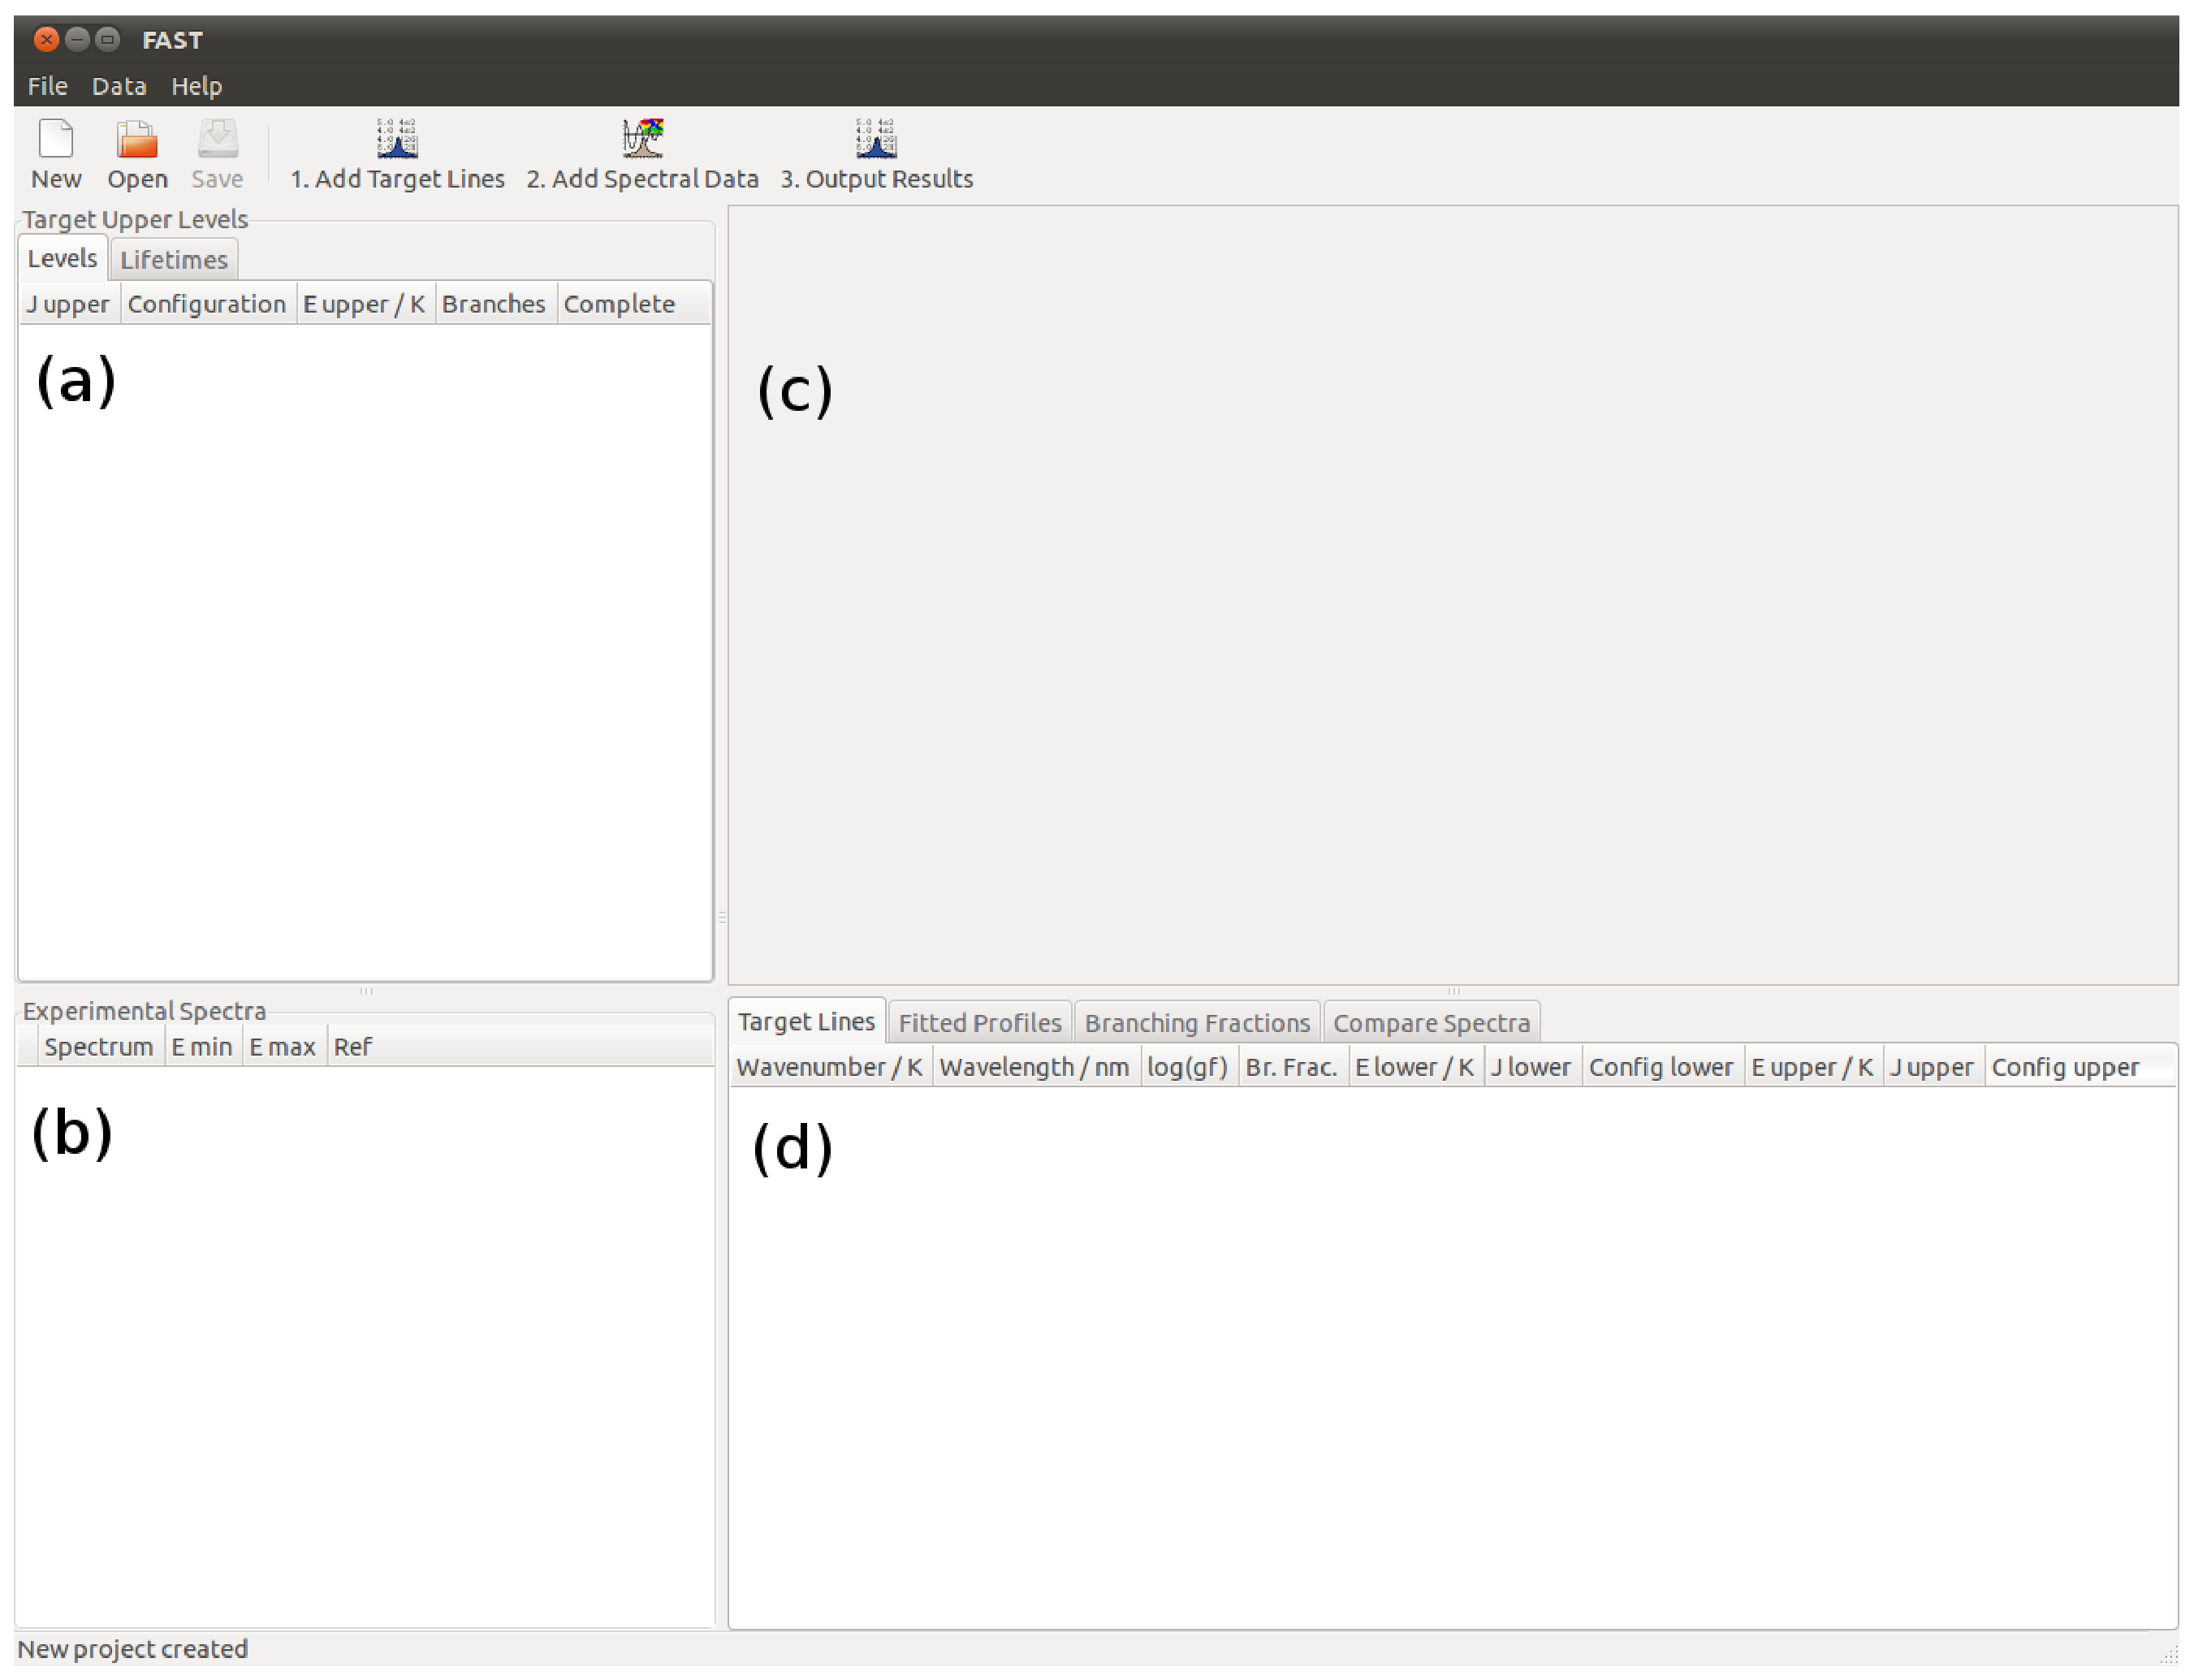
\includegraphics[width=140mm]{fast_new.eps}
\caption{The \fast interface, as seen when first starting the program. The four main window panes, labelled (a) to (d), are resizable to suit the user's needs, and are described in the main text.}
\end{figure}

\section{Examining FT atomic line spectra}

\begin{figure*}\centering
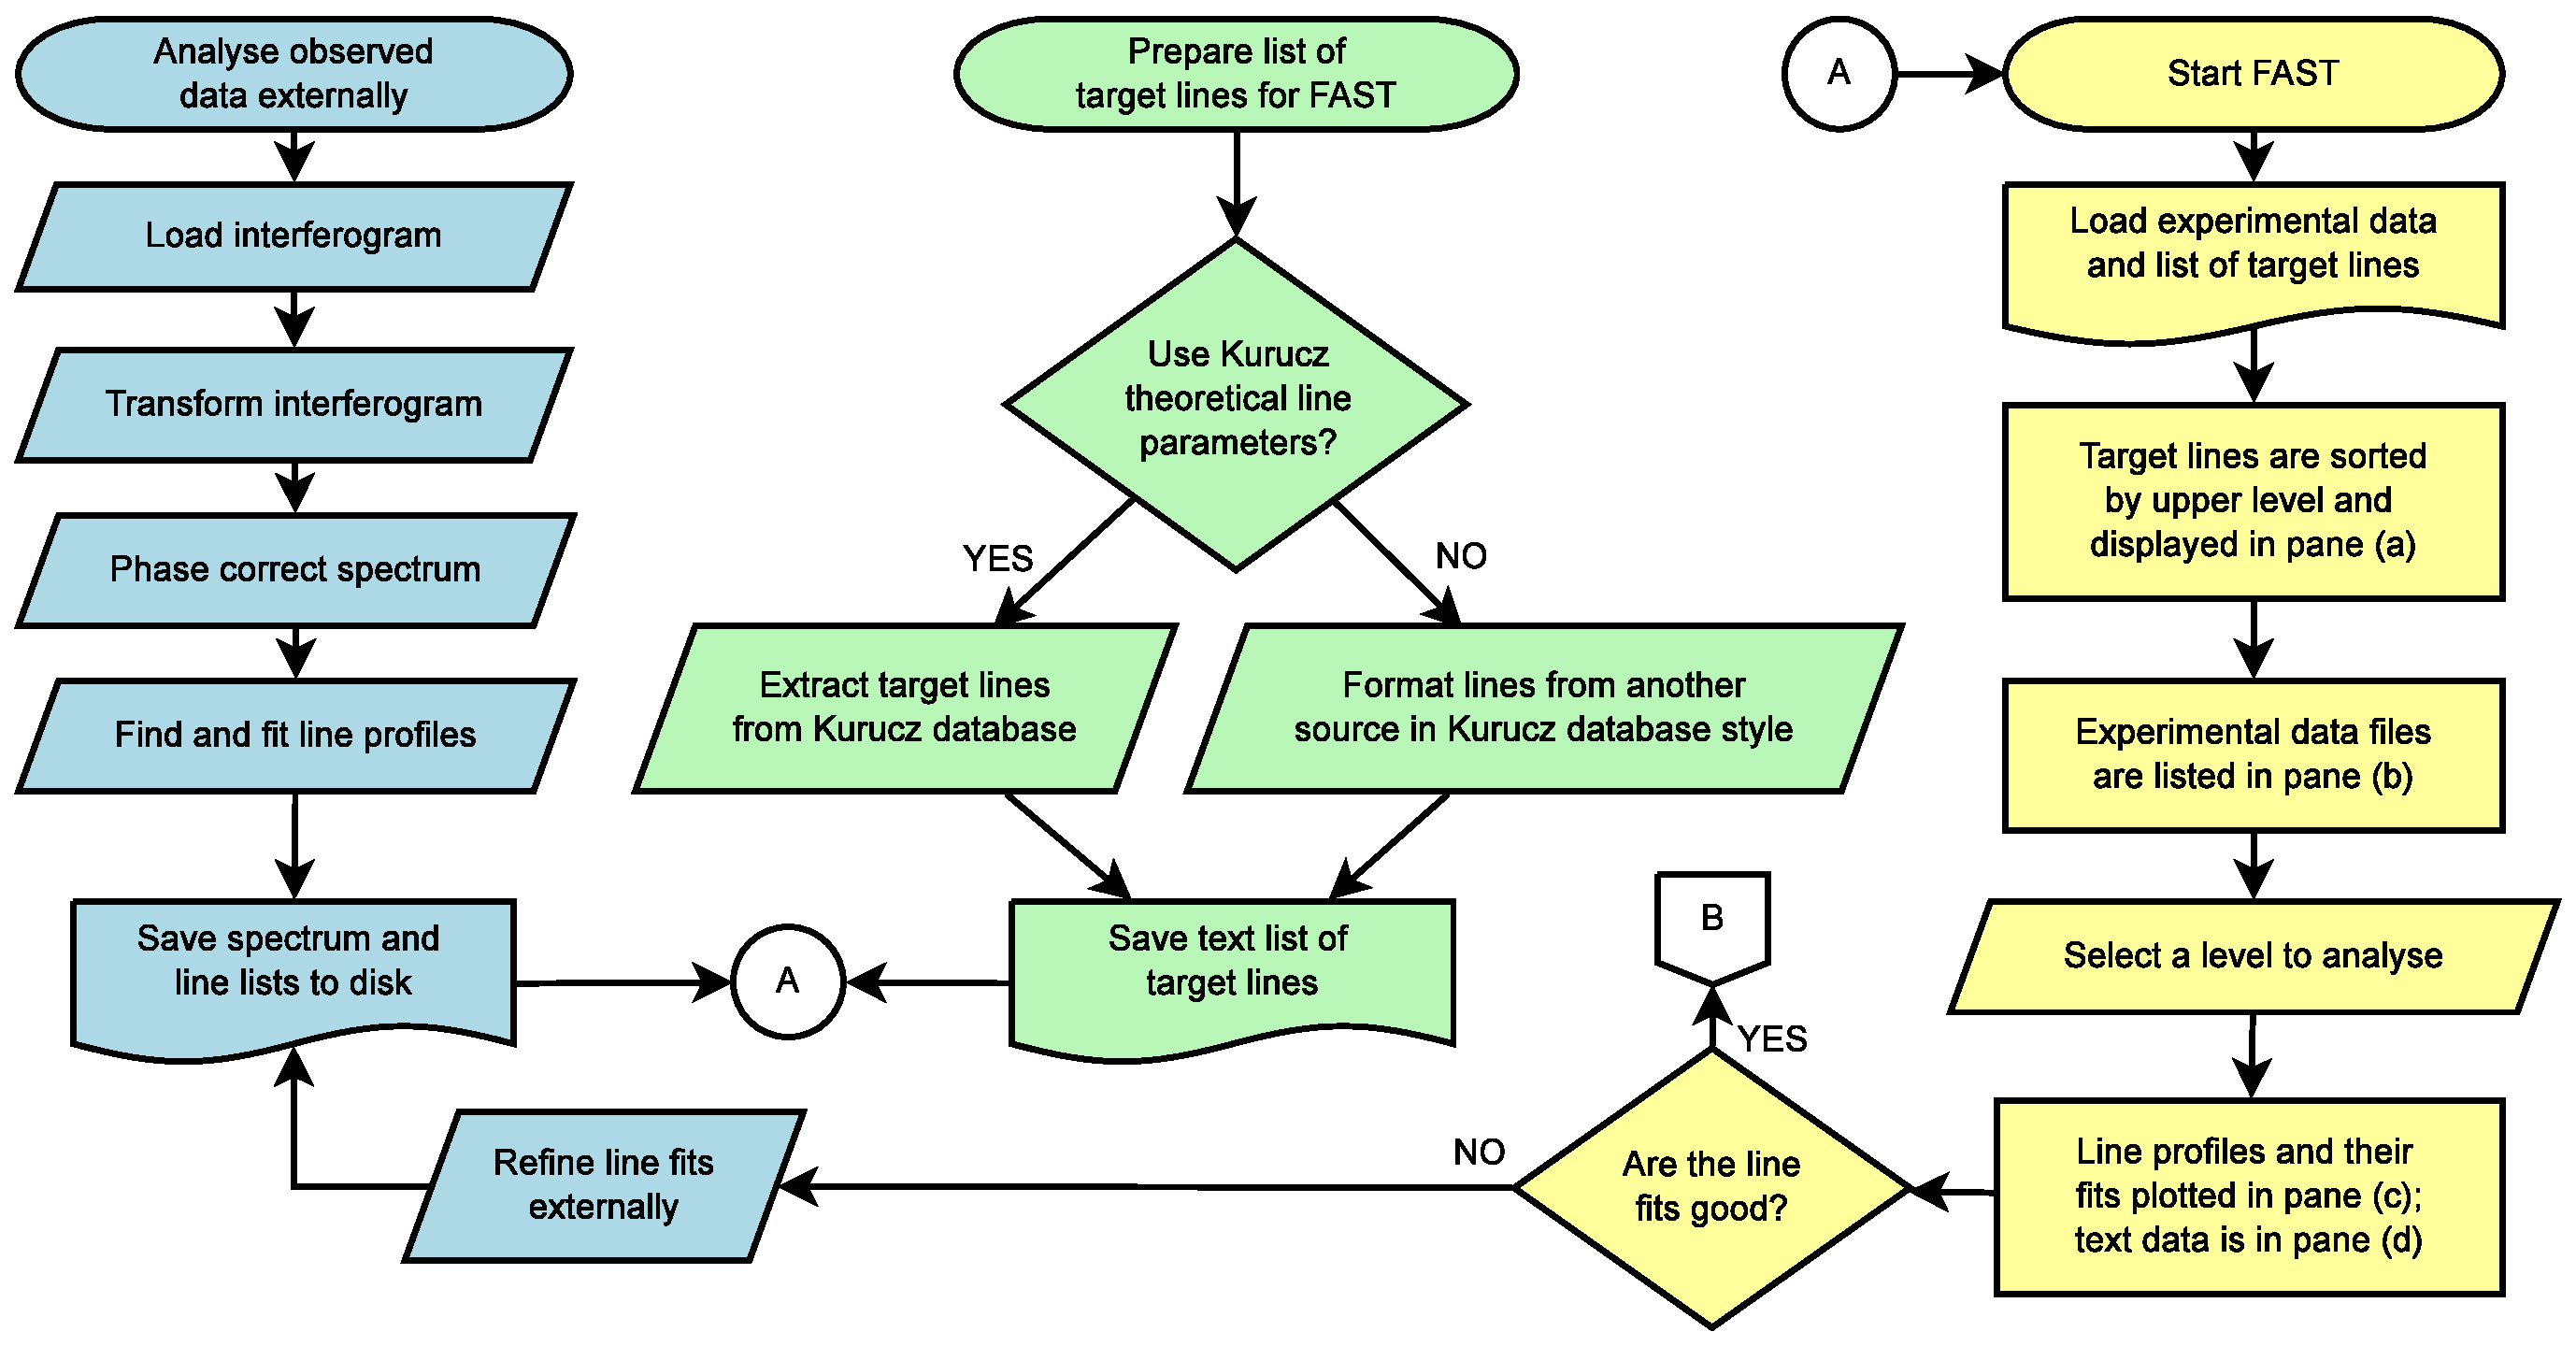
\includegraphics[scale=0.30]{Fast_Flow1.eps}
\caption{Using \emph{FAST} to assist in the analysis of experimental spectra. Those operations in blue are performed in an external, early-stage analysis program such as \emph{XGremlin}, those in green indicate the preparation of a target line list, and those in yellow show the functions performed by \emph{FAST}. The \emph{FAST} interface frames are shown in Figure \ref{fig:gui_new}. `B' links to operations shown in Figure \ref{fig:flow2}.}
\label{fig:flow1}
\end{figure*}

The first primary function of \fast is to allow easy comparison of different experimental and calculated line data. The basic steps to be performed in setting up a \fast project are shown in Figure \ref{fig:flow1}.

\subsection{Specifying which spectral lines to analyse}
The outline of an analysis is specified by loading basic parameters for a number of target lines. These may be obtained from any source, or even generated manually, but given the widespread use of the Kurucz atomic line database (http://kurucz.harvard.edu/), the list of target lines is read into \fast using the same ASCII file format as Kurucz.

These lines of interest are then loaded into \fast by clicking ``Add Target Lines" from the main toolbar or selecting ``Load Target Lines" from the ``Data" menu. A file open dialogue will be displayed, where the text file containing these lines can be selected.

Once loaded the lines will be grouped by upper level in preparation for branching fraction work. These upper levels will be displayed in the ``Target Upper Levels" list in the top-left pane. An upper level can be selected by left-clicking it, after which, the individual lines belonging to it are displayed in the ``Target Lines" tab in the bottom-right pane.

Any number of Target line lists can be loaded into a given \fast project.

\subsection{Adding experimental data}
\label{section:addexptdata}
The easiest way to add experimental data is to click the ``Add Spectral Data" button on the main toolbar. This will bring up a file open dialogue where a measured line spectrum can be loaded. By default, ASCII spectrum files (with a `*.asc' extension) will be displayed. To load a spectrum from an ASCII file, the data should be written in two columns; the first for the wavenumber of the data point (in $cm^-1$) , and the second for its measured intensity. The two should separated by at least one space or tab character. 

\fast is also able to directly load spectra created by the \emph{XGremlin} program. This is done by selecting `XGremlin DAT files' from the dialogue window, and opening the desired spectrum's \verb|.dat| file. As always, a matching \verb|.hdr| file must also be present in the same location. 

Assuming the specified spectrum is loaded correctly, it will be immediately available in the ``Experimental Spectra" list in the bottom-left pane of the \fast window. A second dialogue will then be displayed, asking for a line list. These should be ASCII files formatted follows

\begin{quote}
\begin{verbatim}
# A sample atomic line list. Use # characters for comments
# wavenumber  peak height  width     damping  description
3136.083252   .8675E+00    30.0000   0.0000   a
3161.622070   .7031E+01    30.0000   1.0000   b
3503.436213   .6371E+02    21.3527   0.7853   c
3503.602868   .2055E+02    28.9315   1.0000   d
\end{verbatim}
\end{quote}

However, once again, \xgremlin \verb|.lin| files or ASCII output generated by the \xgremlin \verb|writelines| command may also be read.

Once the line list is loaded, the measured spectrum and fitted line profiles will be available for analysis. Additional line lists can be attached to the spectrum if necessary, as can other types of experimental data, as explained below.

%\subsection{Adding line spectra in isolation}
%To add a new experimental spectrum without automatically attaching a line list to it, either select ``Add Experimental Spectrum" from the ``Data" menu, or right click on a blank space in the ``Experimental Spectra" list and select ``Add New Spectrum" from the popup menu. Select the spectrum you wish to load from the file open dialogue that appears.

\subsection{Attaching additional line lists}
A line list can be attached to any loaded experimental spectrum by right clicking on the target spectrum in the ``Experimental Spectra" list and selecting ``Attach Line List" from the popup menu. Select the line list you wish to load from the file open dialogue that appears.

More than one line list can be added to a given spectrum. This can be particularly useful if you wish to keep different sets of lines separate, such as those belonging to different upper levels.

\subsection{Attaching standard lamp spectra}
If the loaded line spectrum is to be intensity calibrated, both a measured standard lamp spectrum, and its spectral radiance information, must be attached to it. To attach a measured lamp spectrum, right-click on the target line spectrum in the ``Experimental Spectra" list and select ``Attach Standard Lamp Spectrum" from the popup menu. This will display a file open dialogue where the lamp spectrum can be selected.

Only one standard lamp spectrum may be attached to a given line spectrum. If a second standard lamp spectrum is added, it will replace the first.

\subsection{Attaching standard lamp radiance data}
Once a measured standard lamp spectrum has been attached to a spectrum, attach its associated radiance data by right-clicking on the same spectrum in the ``Experimental Spectra" list, and selecting ``Attach Standard Lamp Radiance" from the popup menu. This will display a file open dialogue where the lamp's \verb|.rad| file can be selected. For information on creating \verb|.rad| files, see section \ref{section:radfile}.

Only one set of standard lamp radiance data may be attached to a given line spectrum. If a second \verb|.rad| file is added, it will replace the first.

\subsection{Linking spectra taken simultaneously on different FTS channels}
\label{section:linkspectra}
If two loaded spectra were measured simultaneously, as is the case when measuring from an FT spectrometer's A and B channel together, it can be assumed that both channels saw exactly the same source. Therefore, after intensity calibration, the relative intensity (but not necessarily the signal-to-noise ratios) of any given lines should be identical in both in both spectra. 

This assumption can be useful when trying to put the two spectra on a common absolute intensity scale, especially when channels A and B recorded data in different (but overlapping) spectral ranges as is often the case for branching fraction work. Rather than only using lines from a selected upper level to carry the intensity calibration from one spectrum to the other, \emph{any} line common to both spectra may be used. Since this will typically greatly increase the number of lines over which this intensity scaling factor is determined, the associated uncertainty in linking the two spectra should be significantly lower than for two spectra not recorded simultaneously.

To link two spectra in this way (and thus allow \fast to find the scaling factor needed to put them on a common intensity scale from any line common to both), right click on one of them in the ``Experimental Spectra" list and select ``Link to Another Spectrum" from the popup menu. Then, left-click on the other spectrum. If done correctly, a note will appear in the list of items attached to the second spectrum to say that it is linked to the first.

\section{Working with the loaded data}

\subsection{Viewing target line lists}
Any loaded target lines will be grouped by upper level. These upper levels are then displayed in the ``Target Upper Levels" list in the top-left pane of the \fast window. 

In the ``Levels" tab, basic information about the upper level is displayed; namely its configuration, $J$ value, energy, and the number of branches attached to it. To the right of these, the column ``Complete" indicates the total fraction of the upper level that has been selected from loaded experimental data, which is explained in more detail in section \ref{section:calcbf}. Initially, this will be 0\%. Additional information relating to the upper level is shown in the ``Lifetimes" tab.

To view the individual lines belonging to a given upper level, left-click on that level. The raw target line information will then be displayed in ``Target Lines" tab in the bottom-right pane. In this list, each line will be coloured to indicate its perceived importance to the project.
\begin{itemize}
\item Black text on white: A strong line, found in loaded experimental data.
\item \colorbox{strong_not_found}{Black text on red}: A strong line, not found in any loaded experimental data.
\item \textcolor{weak_found}{Dark grey on white}: A minor line, found in  loaded experimental data.
\item\textcolor{weak_not_found}{Light grey on white}: A minor line, not found in any loaded experimental data.
\end{itemize}

To remove a given upper level from an \fast project, right-click on that level in the ``Target Upper Levels" list and select ``Remove Level" from the popup menu.

\subsection{Manipulating loaded experimental data}
All loaded experimental spectra, and data attached to them, are displayed in the ``Experimental Spectra" list in the bottom-left pane of the \fast window. The spectra are listed in the order in which they were loaded, and are each assigned a letter that is used to reference them elsewhere. Along with the name of the spectrum file, the list includes ``E min" and ``E max" to show the wavenumber range covered by each spectrum. 

A final column on the right of the list, called ``Ref" is used to declare which of the spectra should be used as a reference spectrum. This spectrum will be displayed first when plotting fit profiles and associated textual data. It is also the spectrum that will act as a fixed intensity calibration point when linking overlapping spectra for branching fraction work (see section \ref{section:calcbf}).

Any data attached to a given spectrum will be displayed in a sub-list below it, which is viewed by left-clicking on the arrow next to that spectrum at the very left edge of the list. These additional data files will be colour coded, and will be listed in the following order:

\begin{itemize}
\item \colorbox{attached_line_list}{Yellow background}: Attached line lists. Left clicking on any line list will display all the lines contained in it in the top-right pane of the window and in the ``Fitted Profiles" tab in the bottom-right pane.
\item \colorbox{attached_std_lamp}{Green background}: Attached standard lamp spectrum or spectral radiance data.
\item \colorbox{attached_link}{Blue background}: A note stating that the selected spectrum is linked to another (see section \ref{section:linkspectra}).
\end{itemize}

Any loaded item can be removed by right-clicking on it and selecting the appropriate ``Remove" option in the popup menu that appears. Additional options -- such as attaching more data to a spectrum, or exporting a given set of data to disk -- can also be accessed in these right-click popup menus.

\subsection{Viewing fit profiles and line properties}
When a given upper level is selected in the ``Target Upper Levels" list, any experimental data relating to it will also be displayed. Fitted Voigt profiles for any lines belonging to that level will be displayed in the top-right pane of the window. The raw experimental data will be plotted over these allowing the quality of each fit to be seen at a glance. Beneath each plotted line is a second plot with an expanded vertical scale that shows the fit residuals. Assuming the line has been fitted correctly, its Voigt profile should pass through the measured line profile, with the fit residuals being comparable to the spectral noise. Any artifacts, such as self-absorption, will be visible in the fit residuals in the usual way.

In addition to this, the Voigt profile fit parameters are displayed in the ``Fitted Profiles" tab in the bottom-right pane. In addition to the fit parameters, the first column on this list displays a letter, indicating which of the experimental spectra the line parameters correspond to. If a given line is observed in more than one experimental spectrum, the properties of the line belonging to the reference spectrum will be displayed first, with the fit parameters from other spectra available by expanding the list view beneath it.

In this list of experimental data, the background of the ``Intensity" column will be coloured \colorbox{int_not_calibrated}{red} if there is insufficient standard lamp data attached to a given spectrum to intensity calibrate it. In this case, the displayed integrated line intensities are those determined from the Voigt profile fits alone. If, however, the box is coloured \colorbox{int_calibrated}{green}, the intensity of that line has been calibrated using both the measured standard lamp spectrum and radiance data attached to that spectrum. The integrated intensity shown will therefore have been adjusted to compensate for the instrument response.

\section{Saving and loading \fast projects}
A project may be saved at any time by clicking the ``Save" button on the toolbar, or by selecting ``Save" or ``Save as" from the ``File" menu. \fast will include all imported data files in its own \verb|.fts| file, so it is not strictly necessary to keep all the raw data at the end of an analysis\footnote{although it's obviously advisable not to delete important data!}.

Previously saved projects may be loaded by clicking the ``Open" button on the toolbar, or by selecting ``Open" from the ``File" menu. Loading a project will replace the current project environment.

\section{Exporting data sets to disk}
When data files are added to an \fast project, their contents is stored in \emph{FAST}'s own \verb|.fts| project file. As a result, they can be exported back to disk if necessary, such as for further analysis in an external package.

To export all data files associated with the current project, select ``Export Project" from the ``File" menu. You will be prompted for the name of a folder into which all the data will be saved. Experimental data shown in the ``Experimental Spectra" list will be saved to that location under their original file names. Target line data will be saved in a file called ``targets.txt".

To export a single experimental data file to disk, right-click on it in the ``Experimental Spectra" list and select the appropriate ``Export" option from the popup menu.

\chapter{Advanced Analysis Features}

\begin{figure*}\centering
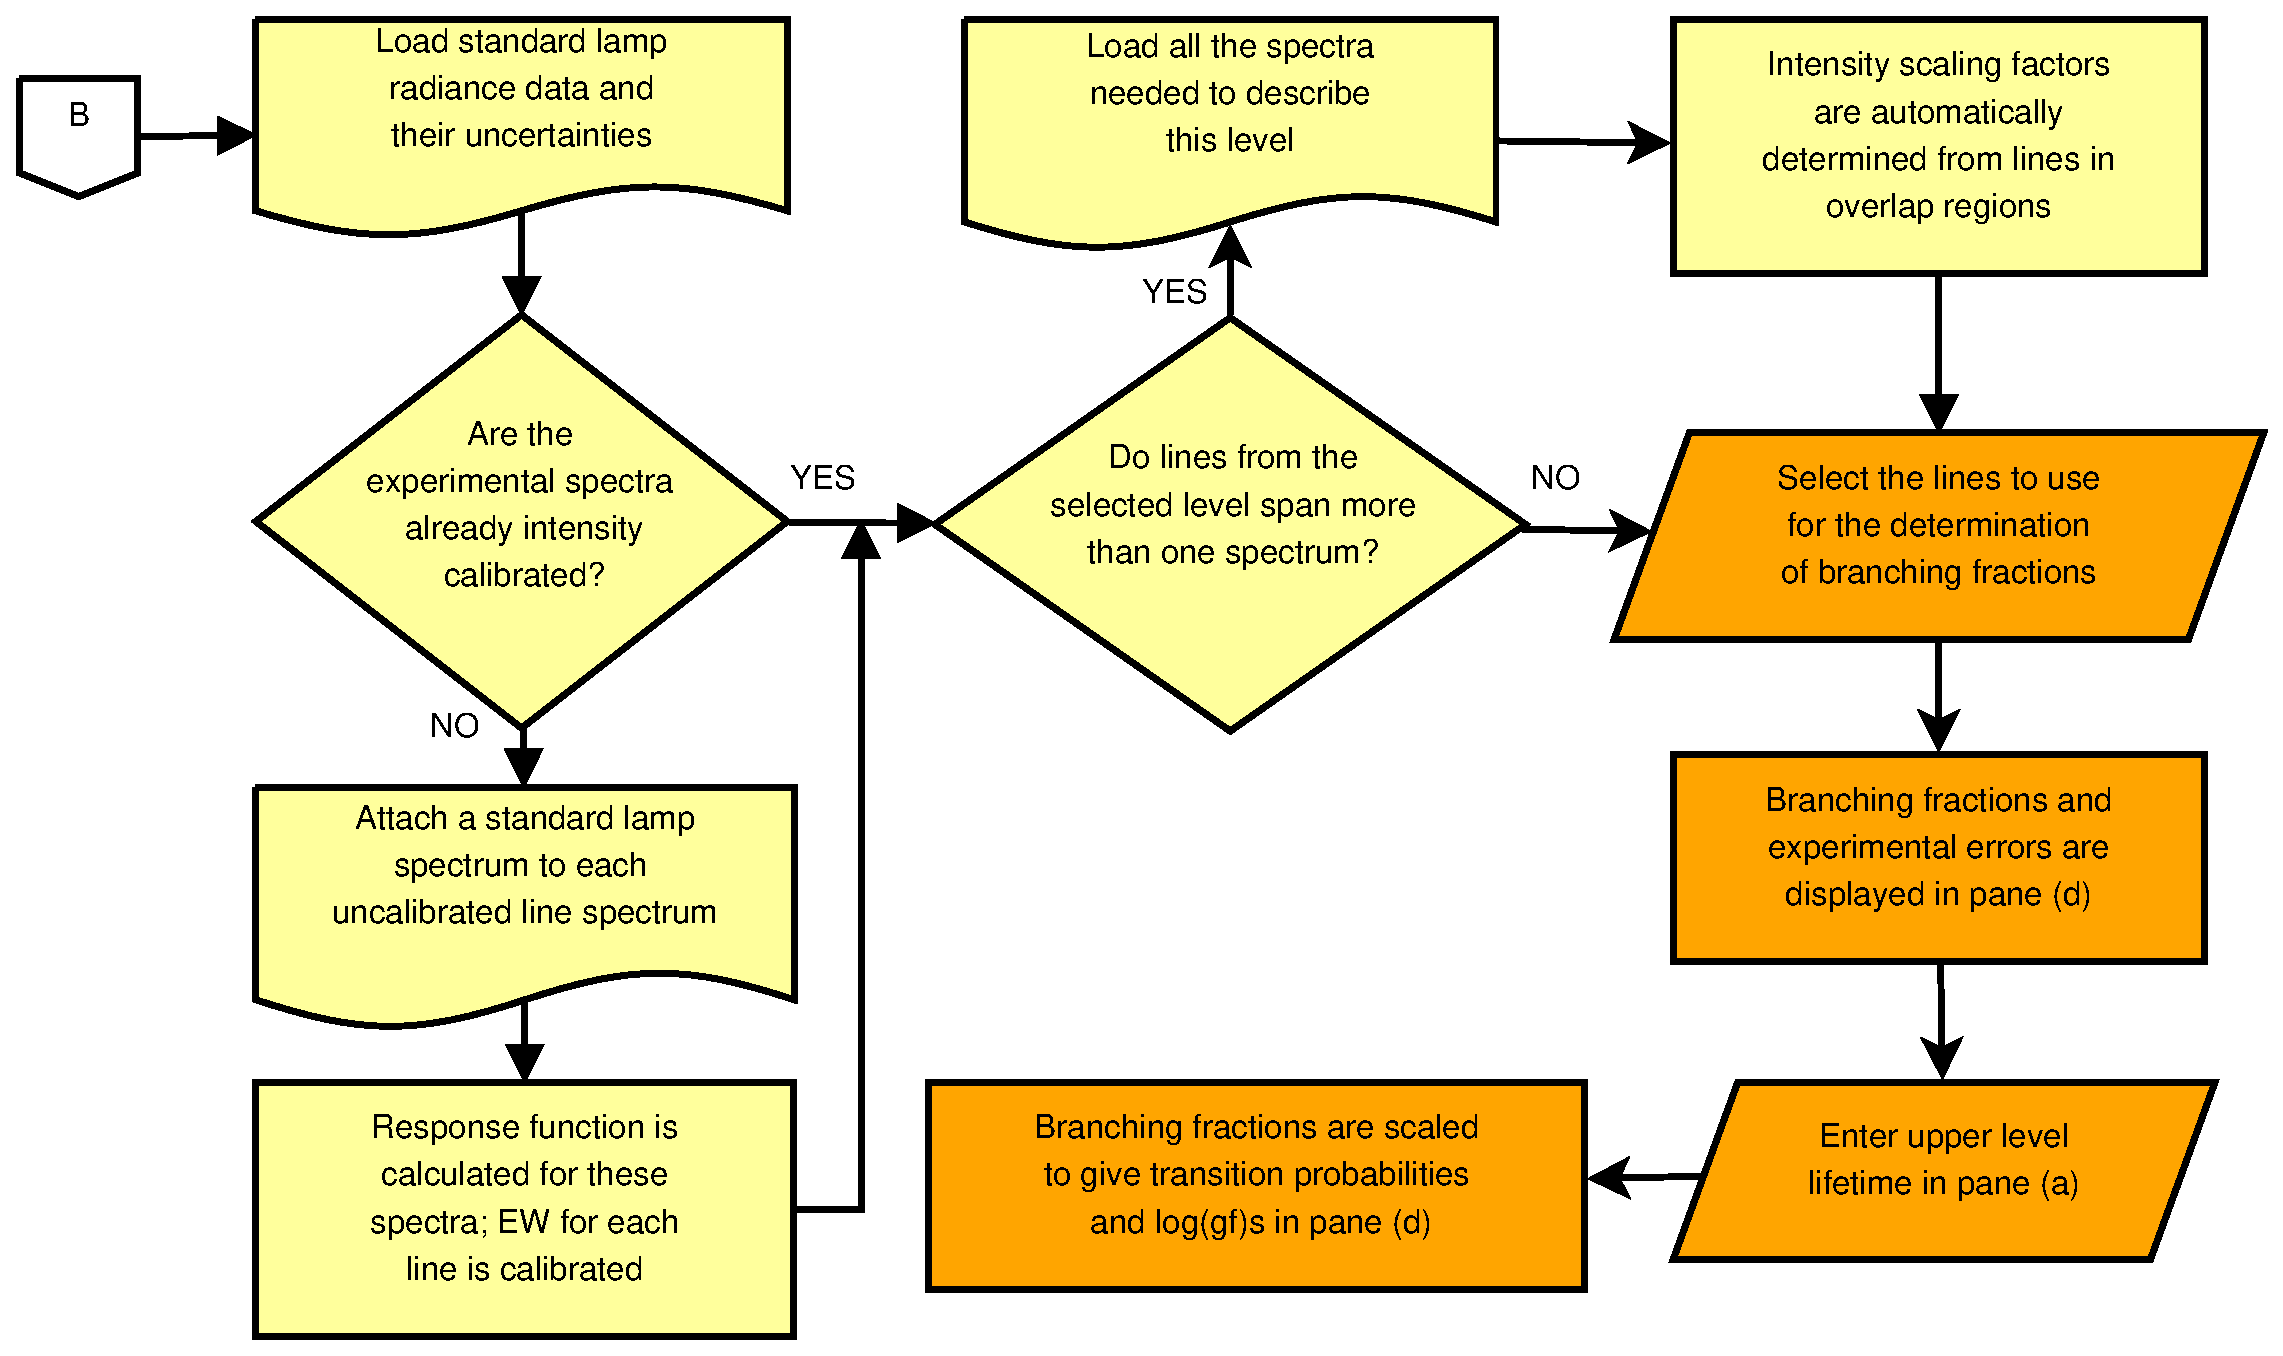
\includegraphics[scale=0.30]{Fast_Flow2.eps}
\caption{Using \emph{FAST} to determine atomic branching fractions, transition probabilities, and oscillator strengths. These operations are performed after those listed in Figure \ref{fig:flow1}. The steps shown in yellow are for intensity calibration of the line spectra and the linking of overlapping spectral regions; those in orange show the final steps, during which the $BF$, $A$, and $\log(gf)$ values are obtained.}
\label{fig:flow2}
\end{figure*}

\section{Spectrum intensity calibration}
\label{section:intcal}

\subsection{Data needed for intensity calibration}
To intensity calibrate a line spectrum, the response function of the spectrometer must be known. This function can be found by comparing the measured spectrum of a calibrated standard lamp with its known spectral radiance. Thus, two additional sets of data must be attached to each line spectrum along side its line lists, as shown in Figure \ref{fig:flow2}.
\begin{itemize}
\item The spectrum of a standard lamp covering the same wavenumber region as the line spectrum itself. \fast will import this from a two-column ASCII file, there the first column specifies the wavenumber of a data point, and the second the measured intensity.
\item The spectral radiance of this same lamp, read from a \verb|.rad| file (see section \ref{section:radfile}, below).
\end{itemize}
Once both of these files are present, \fast will automatically calculate the spectrometer response function at the time the spectrum was taken, and correct for it when displaying the integrated intensity of each of the lines belonging to that spectrum. To indicate that this correction is being applied, the background colour of the integrated intensities listed in the ``Fitted Profiles" and ``Branching Fractions" tabs in the bottom-right pane, and the ``I observed" and ``I normalised" columns in the ``Lifetimes" tab in the top-left pane, will change to \colorbox{int_calibrated}{green}. If no intensity calibration is applied, the background will be \colorbox{int_not_calibrated}{red}.

If an imported line spectrum has already been intensity calibrated, do not attach a measured standard lamp spectrum to it. This will prevent \fast from applying a second, erroneous intensity calibration. However, you should still attach a \verb|.rad| file to the spectrum, as this will tell \fast about the uncertainty in line intensities that comes from the calibration of the standard lamp.

\subsection{Generating a spectral radiance file}
\label{section:radfile}
A spectral radiance \verb|.rad| file is very straightforward to generate. At the top of the file, two columns of data should be specified; the first for a wavelength in nm (\emph{not} a wavenumber), and the second for the measured spectral radiance at that wavelength. The two columns should be separated by a space or tab character.

Immediately beneath this should be a line containing an upper case U as the first character. This defines the start of the radiance uncertainties section. Here, three columns are needed; the first two define a minimum and maximum wavelength and thus a range over which an uncertainty applies, the third contains the percentage uncertainty in spectral radiance in that range.

Any line beginning with a `\#' character will be treated as a comment.

A full example is given below:

\begin{quote}
\begin{verbatim}
# A sample spectral radiance RAD file.
# First give the spectral radiance data
# wavelength / nm      radiance
  1000.0               136.
  1050.0               137.
  1100.0               136.
  1200.0               128.
U
# Then give the calibration uncertainties
# lambda min     lambda max    uncertainty / %
  1000.0         1200.0        1.1
\end{verbatim}
\end{quote}

\section{Branching fractions and log(gf)s}
\subsection{Finding branching fractions and log(gf)s}
\label{section:calcbf}
The steps involved in determining branching fractions are shown in orange in Figure \ref{fig:flow2}. The experimental spectra should first have been intensity calibrated, as explained above in section \ref{section:intcal}. Once this is done, the target upper level should be selected in the ``Target Upper Levels" list. As usual, the experimental line profiles associated with this level will be displayed in the top-right pane of the window. The layout of these plots is very important.

Plots in a given row are obtained from the same experimental spectrum. Plots in a given column are all related to the same upper level branch. Thus, reading across the plot window you will see all the different lines for the selected upper level in a given spectrum, and reading down the plot window you will see the same line as observed in several different spectra. In order to maintain this grid, a blank space is left whenever a line is missing from a given spectrum.

Plots associated with the selected reference spectrum will be displayed in the first row of the plot table, as, by implication, they are the most important for finding the branching fraction. Typically the reference spectrum will contain most of the branches from the selected upper level, and have the best signal-to-noise ratio. 

For two different, but overlapping spectra used to find a given set of branching fractions, there must (as always) be at least one common line. Therefore, to link a second spectrum to the reference, at least one column must be filled for both of them. The same rule holds for linking a third spectrum to the second, and so on. 

If there are no common lines between two spectra, they cannot be linked and so should not be used together when finding branching fractions. The only exception applies when two spectra are linked, as described in section \ref{section:linkspectra}. In this case, a transfer factor can be determined from lines that are not part of the selected upper level.

Assuming that all the required spectra can be linked correctly, left-click on the plots of the lines that are to be included when determining the branching fractions. Once selected in this way, their background will turn blue. If necessary, left-click them again to unselect them. Where a line is observed in more than one spectrum, select the line from the spectrum where is has the greatest signal-to-noise ratio. At the end of this procedure exactly one line should have been selected in each column for all the transitions to be used.

As each line is selected, its associated branching fraction data will appear in the ``Branching Fractions" tab in the bottom-right pane. Data shown in the ``Lifetimes" tab in the top-left pane will also be updated, and the percentage shown in the ``Complete" column of the ``Levels" tab will increase by the amount the line is predicted to contribute to the total upper level transition probability. This prediction is based on the $\log(gf)$s specified in the loaded list(s) of target lines. Ideally, once all the target branches have been selected, this percentage should be close to 100\%. At this point, the branching fractions shown in the ``BF" column of the ``Branching Fractions" list are found using
\begin{equation}
\label{eqn:bfexpt}
BF_i = \frac{I_i}{\sum_i{I_i} + I_{missing}}~,
\end{equation}
where $I_{missing}$ is the sum of predicted integrated intensities for the unobserved branches, obtained from the list of target lines. Again, the integrated intensities shown in the ``Branching Fractions" list will be coloured \colorbox{int_not_calibrated}{red} if they are not intensity calibrated, or \colorbox{int_calibrated}{green} if they are.

With the individual ($BF_i$) known, they can be combined with the upper level lifetime in the usual way to obtain the associated transition probabilities ($A_i$), which are shown in the ``A" column.
\begin{equation}
A_i = \frac{BF_i}{\tau_u}~.
\end{equation}
$\tau_u$ and its associated uncertainty, $\Delta\tau_u$, may be specified in the ``Lifetimes" tab in the top-left pane. It then follows that the $\log(g_lf)_i$ values (shown in the ``log(gf)" column) are
\begin{equation}
\log(g_lf)_i = \log\Bigl[A_i(g_u \lambda^2)_i\times 1.499\times 10^{-14} \Bigr]
\end{equation}

\subsection{Uncertainties in branching fractions and log(gf)s}
To determine the experimental uncertainties in branching fractions and log(gf)s, several sources or error must be taken into account
\begin{itemize}
\item $U_{i(S/N)_l}~(\%)$: The intensity uncertainty of line $i$, which is the inverse of its signal-to-noise ratio.
\item $U_{i(S/N)_r}~(\%)$: The intensity uncertainty of the measured standard lamp spectrum at the same wavenumber as line $i$.
\item $U_{i(cal)}~(\%)$: The uncertainty in the standard lamp spectral radiance at the same wavenumber as line $i$.
\item $U_{i(trans)}~(\%)$: The uncertainty in scaling the intensity of line $i$ to put it on the same intensity scale as lines in another spectrum. By definition, this will be zero for the reference spectrum, and will be progressively larger for each spectrum linked in a chain back to it.
\end{itemize}

$U_{i(S/N)_l}$, $U_{i(cal)}$, and $U_{i(trans)}$ are displayed in the ``Branching Fractions" list. $U_{i(S/N)_r}$ is usually very small and so is added in quadrature to the displayed value of  $U_{i(cal)}$. If no spectral radiance data has been added to a given spectrum, $U_{i(cal)}$ for its lines will be zero, and when displayed in the ``U(cal)" column, their background will be \colorbox{int_not_calibrated}{red}. If spectral radiance data is available, the background will be \colorbox{int_calibrated}{green}.

All these uncertainties are added in quadrature to give a total error in the intensity of line $i$, which is shown in the ``U(total)" column.
\begin{equation}
U_i~(\%) = \sqrt{U^2_{i(S/N)_l} + \Biggl(\frac{U_{i(cal)}}{\sqrt{2}}\Biggr)^2 + U^2_{i(S/N)_r} + U^2_{i(trans)}}~.
\end{equation}
With $U_i$ known, the uncertainty in each line's integrated intensities (shown in the ``U(Int.)" column) may be found
\begin{equation}
\Delta I_i = I_i\times \frac{U_i}{100}~,
\end{equation}
which is then summed with all other $\Delta I_i$ to give a total uncertainty in the selected upper level's integrated intensity.
\begin{equation}
\Delta I_{total} = \sqrt{\sum_i\Delta I^2_i}~.
\end{equation}
From this, it follows that the uncertainty in a line's branching fraction (shown in the ``U(BF)/\%" column) is
\begin{equation}
\Delta BF_i~(\%) = \sqrt{\Biggl(\frac{100\times\Delta I_{total}}{I_{total}}\Biggr)^2 + U_i^2}~,
\end{equation}
which, when combined with the uncertainty in the upper level's lifetime, $\Delta\tau_u$, gives the uncertainty in the line's transition probability (shown in the ``U(A)/\%" column).
\begin{equation}
\Delta A_i~(\%) = \sqrt{\Delta BF_i^2 + \Biggl(\frac{100\times \Delta\tau_u}{\tau_u}\Biggr)^2}~.
\end{equation}
Finally, the uncertainty in $\log (g_uf)_i$ (shown in the ``dex" column) is
\begin{equation}
\Delta\log (g_uf)_i~(\mbox{dex}) = \log\Biggl[(g_uf)_i + \Biggl((g_uf)_i \times \frac{\Delta A_i}{100}\Biggr)\Biggr] - \log[(g_uf)_i]~.
\end{equation}

\chapter{An Example}
\section{The example files}
Along with this document, you should find a folder called `example'. On Linux-based systems, this will likely be located in `/usr/share/doc/fast', but can also be downloaded separately from the \fast website. In this folder are the following files.

\begin{itemize}
\item \verb|example.fts| - An example \fast project created from the files listed below. This chapter will explain how to create this project.
\item \verb|targets.txt| - A list of target lines for analysis.
\item \verb|ascii_spectrum.asc| - A two-column ASCII file containing a sample spectrum.
\item \verb|ascii_line_list.asc| - A \fast ASCII line list containing fits to some lines in \verb|ascii_spectrum.asc|.
\item \verb|ascii_writelines.asc| - An XGremlin generated ASCII line list containing the same data as \verb|ascii_line_list.asc|.
\item \verb|xg_spectrum.dat| - An XGremlin spectrum containing the same sample spectrum as \verb|ascii_line_list.asc|.
\item \verb|xg_spectrum.hdr| - An XGremlin header file for \verb|xg_spectrum.dat|.
\item \verb|xg_spectrum.lin| - An XGremlin line list containing the same data as \verb|ascii_line_list.asc|.
\item \verb|standard_radiance.rad| - A standard lamp spectral radiance file. Its contents is described in section \ref{section:radfile}.
\item \verb|standard_spectrum.asc| - An ASCII file containing an observation of the standard lamp described in \verb|standard_radiance.rad|.
\end{itemize}

\section{Creating the `example.fts' project}

First open a terminal window and go to the `/usr/share/doc/fast/example' folder (if you downloaded the example separately, go to the location you have extracted it to instead). Start \fast by running \verb|fast|. Once the main window appears follow the steps shown in each of the following figures. By the end, you should have created the same project saved in `example.fts'.
\newpage
\begin{figure}\centering
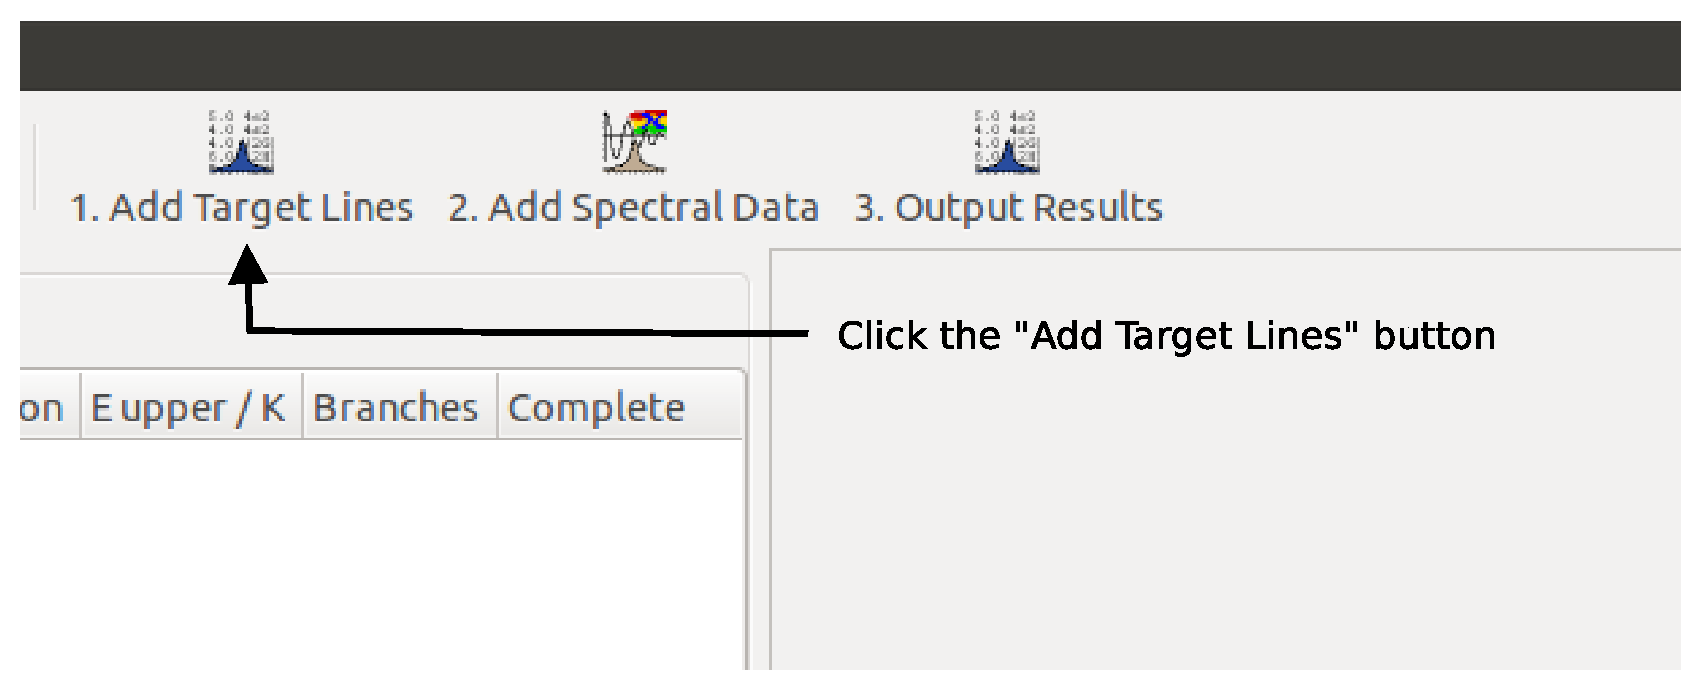
\includegraphics[scale=0.37]{Tutorial1.eps}
\caption{Once \fast has loaded, click the ``Add Target Lines" button from the main toolbar.}
\label{fig:tut1}
\end{figure}

\begin{figure}\centering
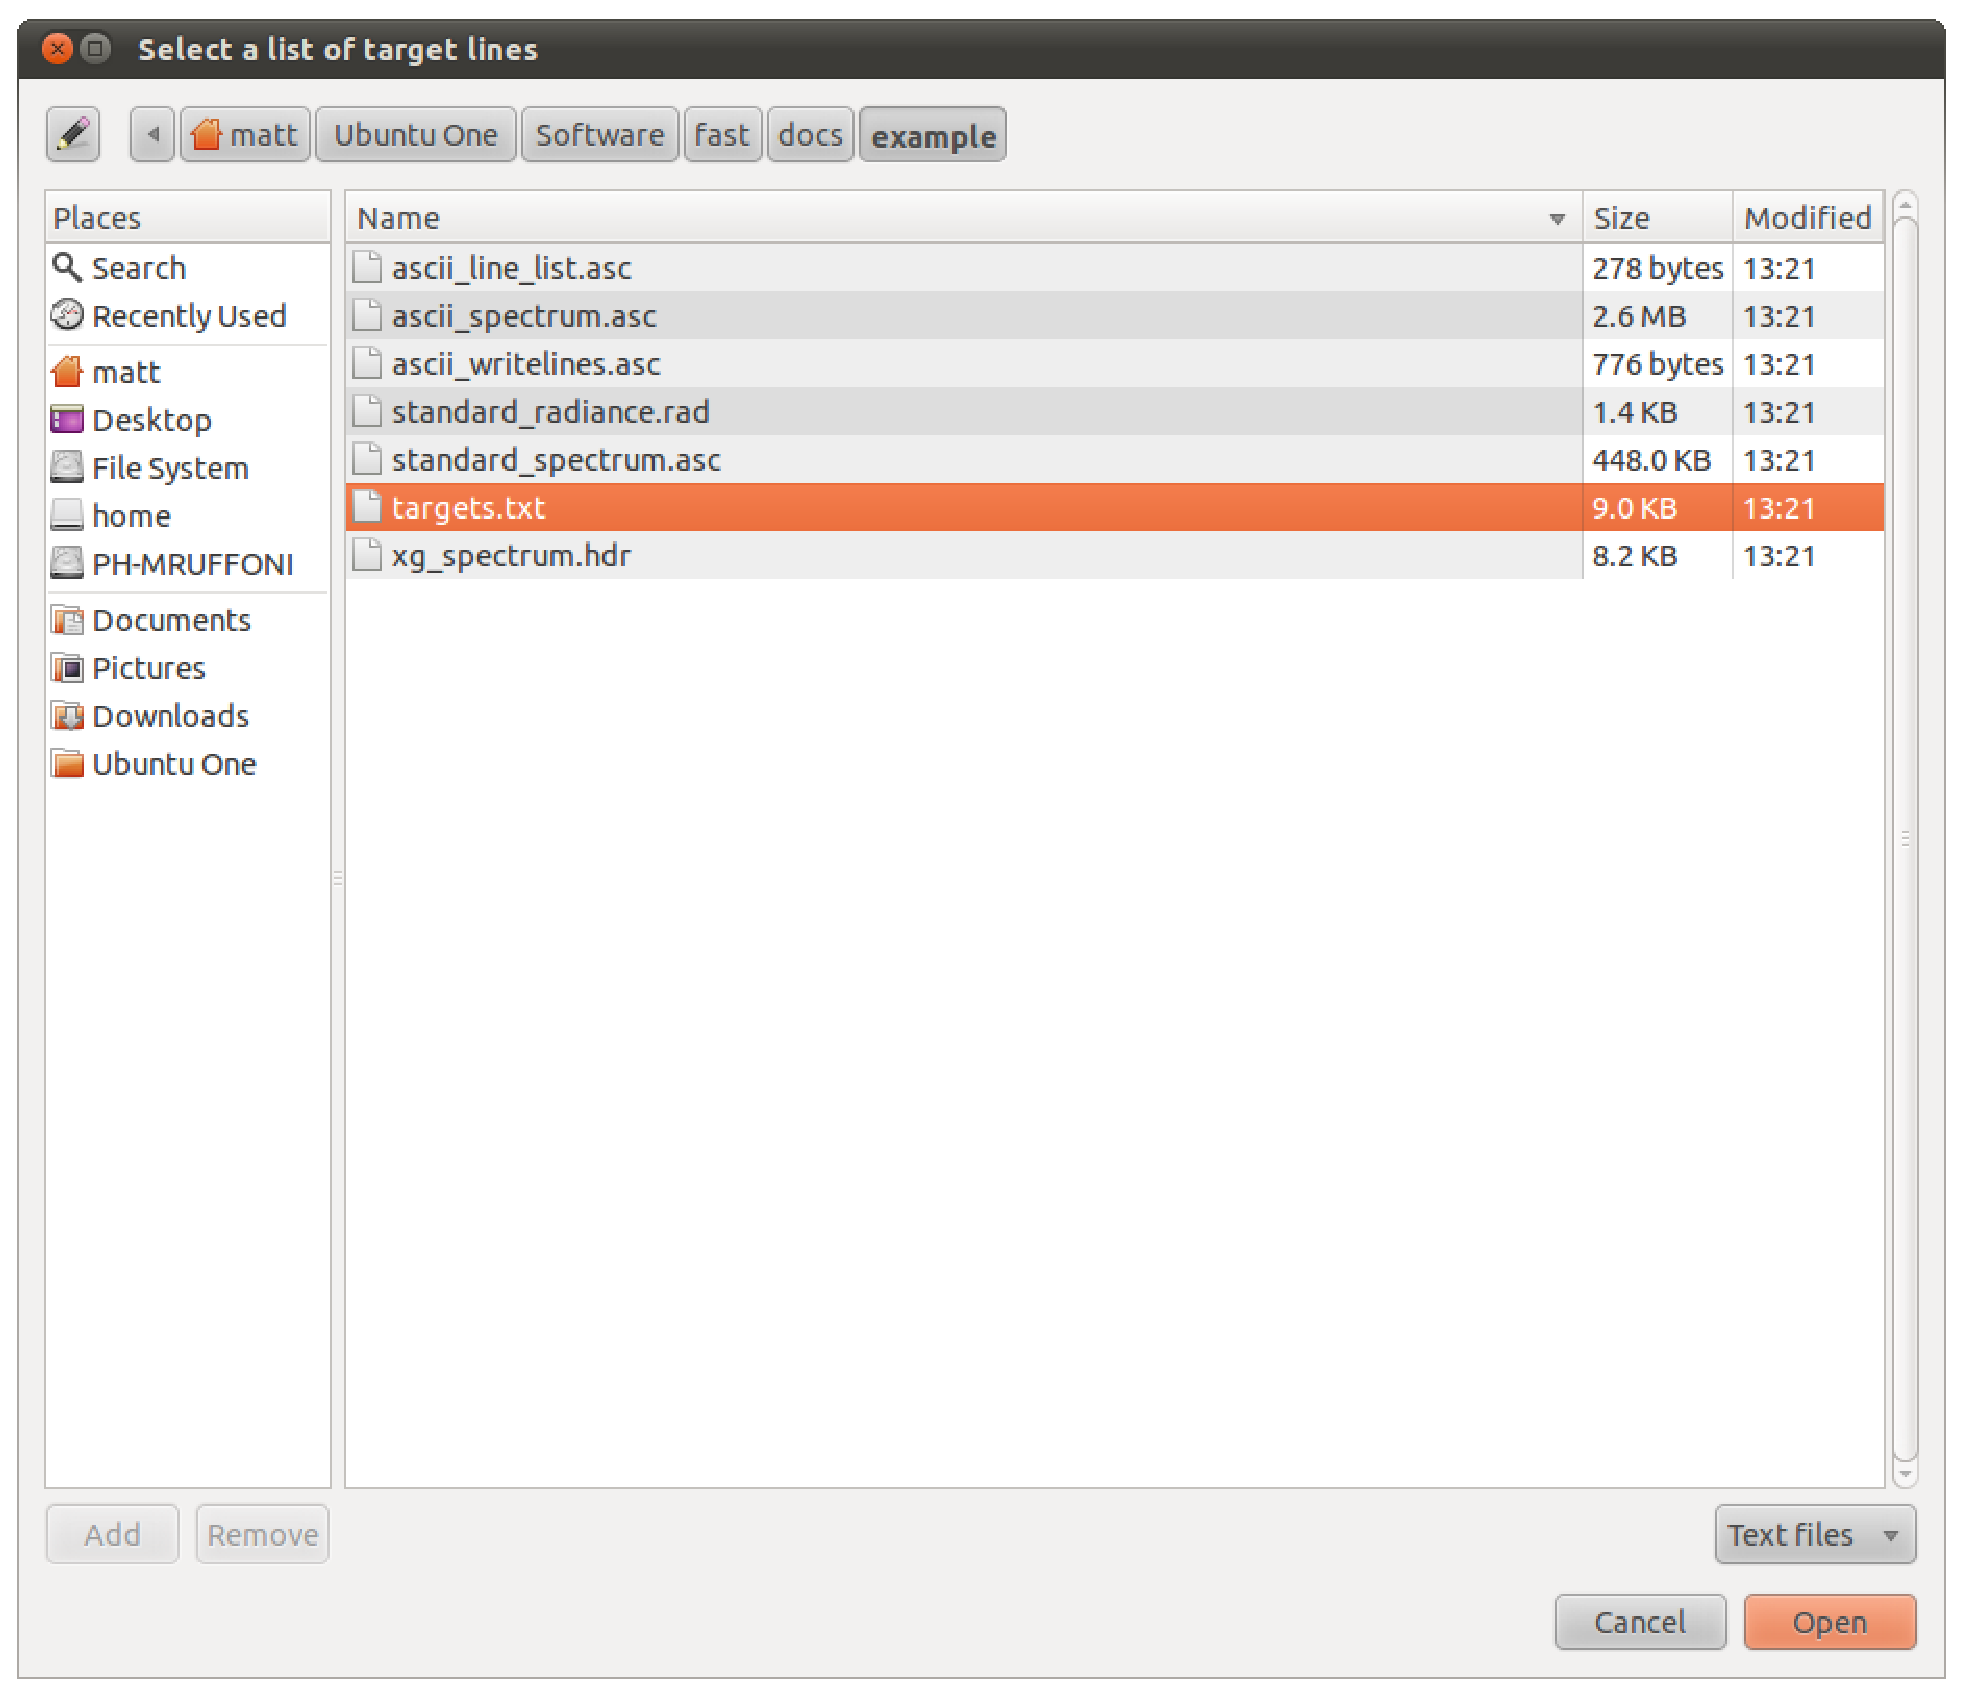
\includegraphics[width=140mm]{Tutorial2.eps}
\caption{A file open dialog will pop-up asking for a list of target lines. Select `targets.txt' from the list of files in the example folder, and click `Open'.}
\label{fig:tut2}
\end{figure}

\begin{figure}\centering
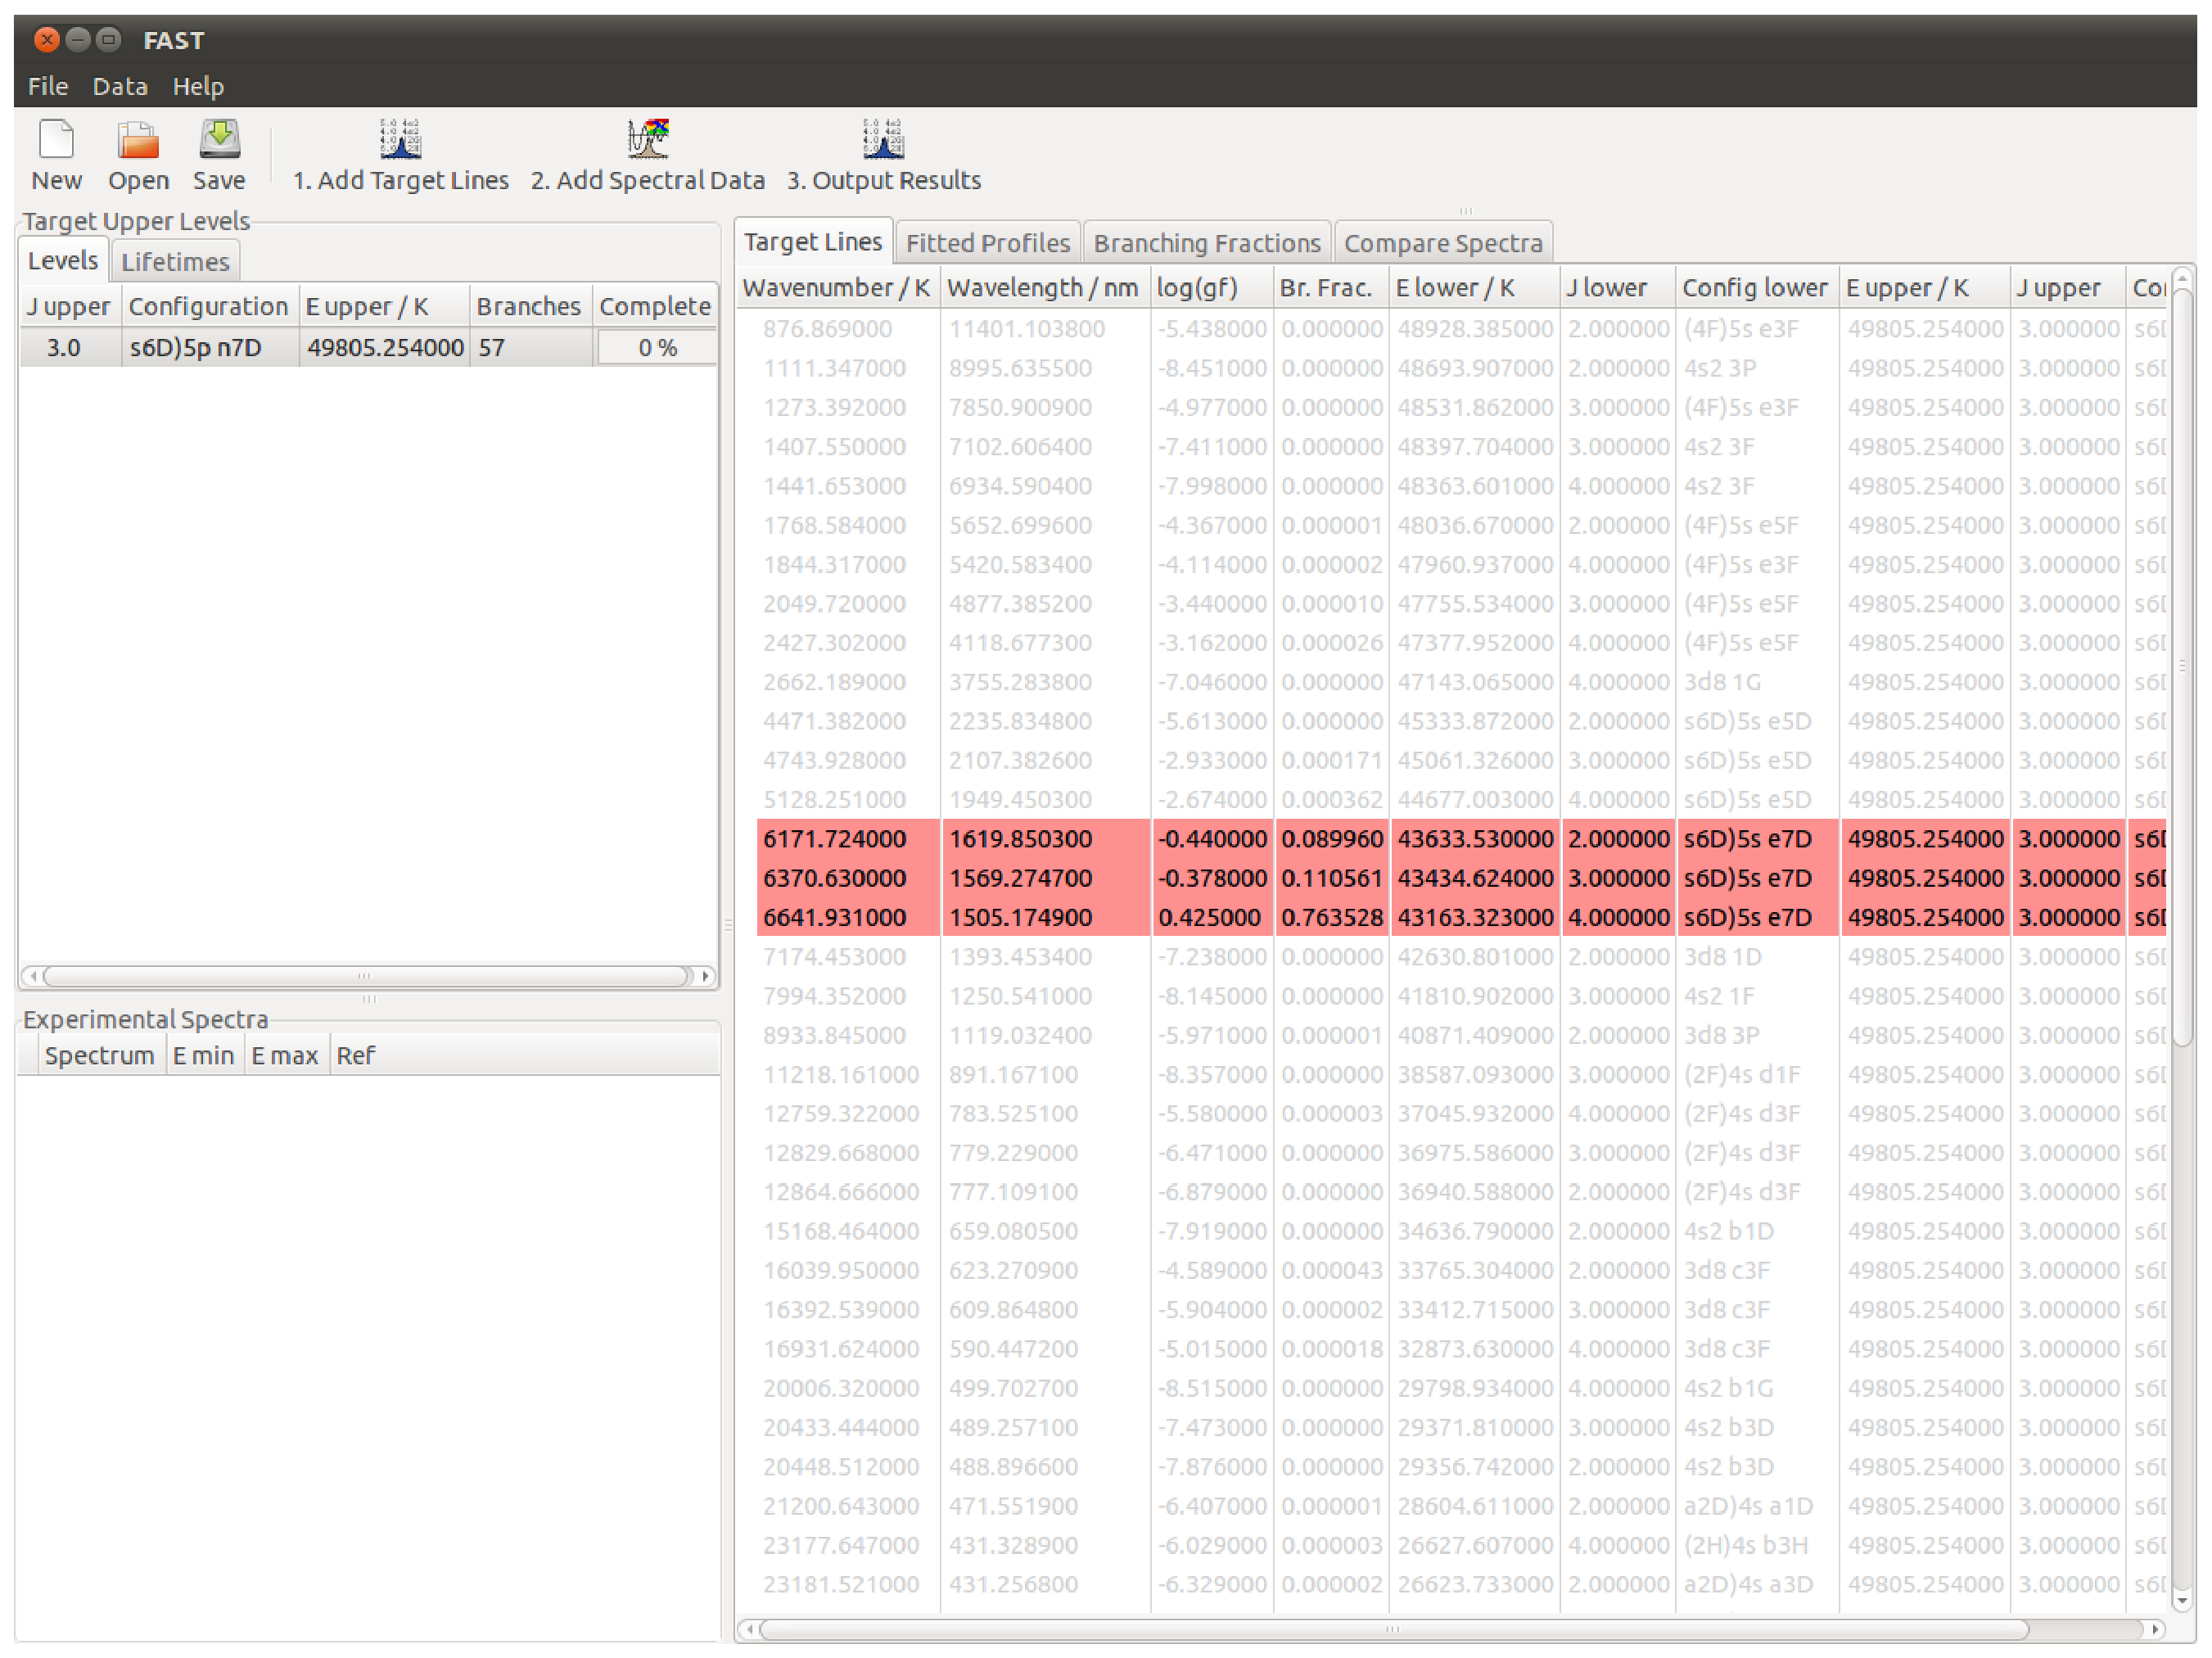
\includegraphics[width=140mm]{Tutorial3.eps}
\caption{The contents of `targets.txt' is read by \emph{FAST}. It contains the transitions associated with a single upper level. This level is listed in pane (a). Click on it to view the individual transitions in pane (d). All the panes can be resized by dragging their borders. Drag the top of pane (d) upwards to view more transitions.}
\label{fig:tut3}
\end{figure}

\begin{figure}\centering
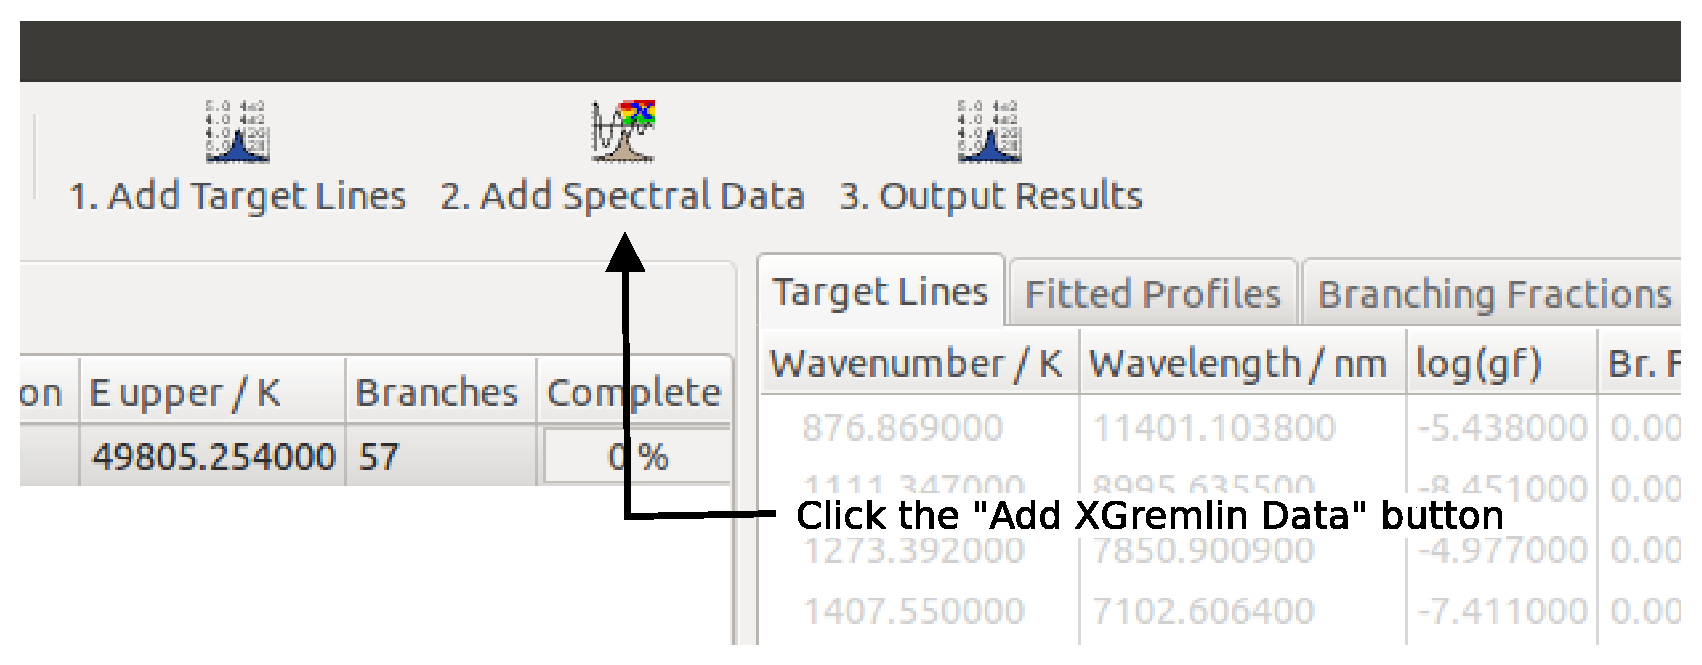
\includegraphics[scale=0.37]{Tutorial4a.eps}
\caption{Next, the experimental data needs to be loaded. Click the ``Add Spectral Data" button on the main toolbar.}
\label{fig:tut4a}
\end{figure}

\begin{figure}\centering
\includegraphics[width=140mm]{Tutorial4.eps}
\caption{A file open dialog will pop-up asking for an experimental data file. Select 'ascii\_spectrum.asc' and click `Open'.}
\label{fig:tut4}
\end{figure}

\begin{figure}\centering
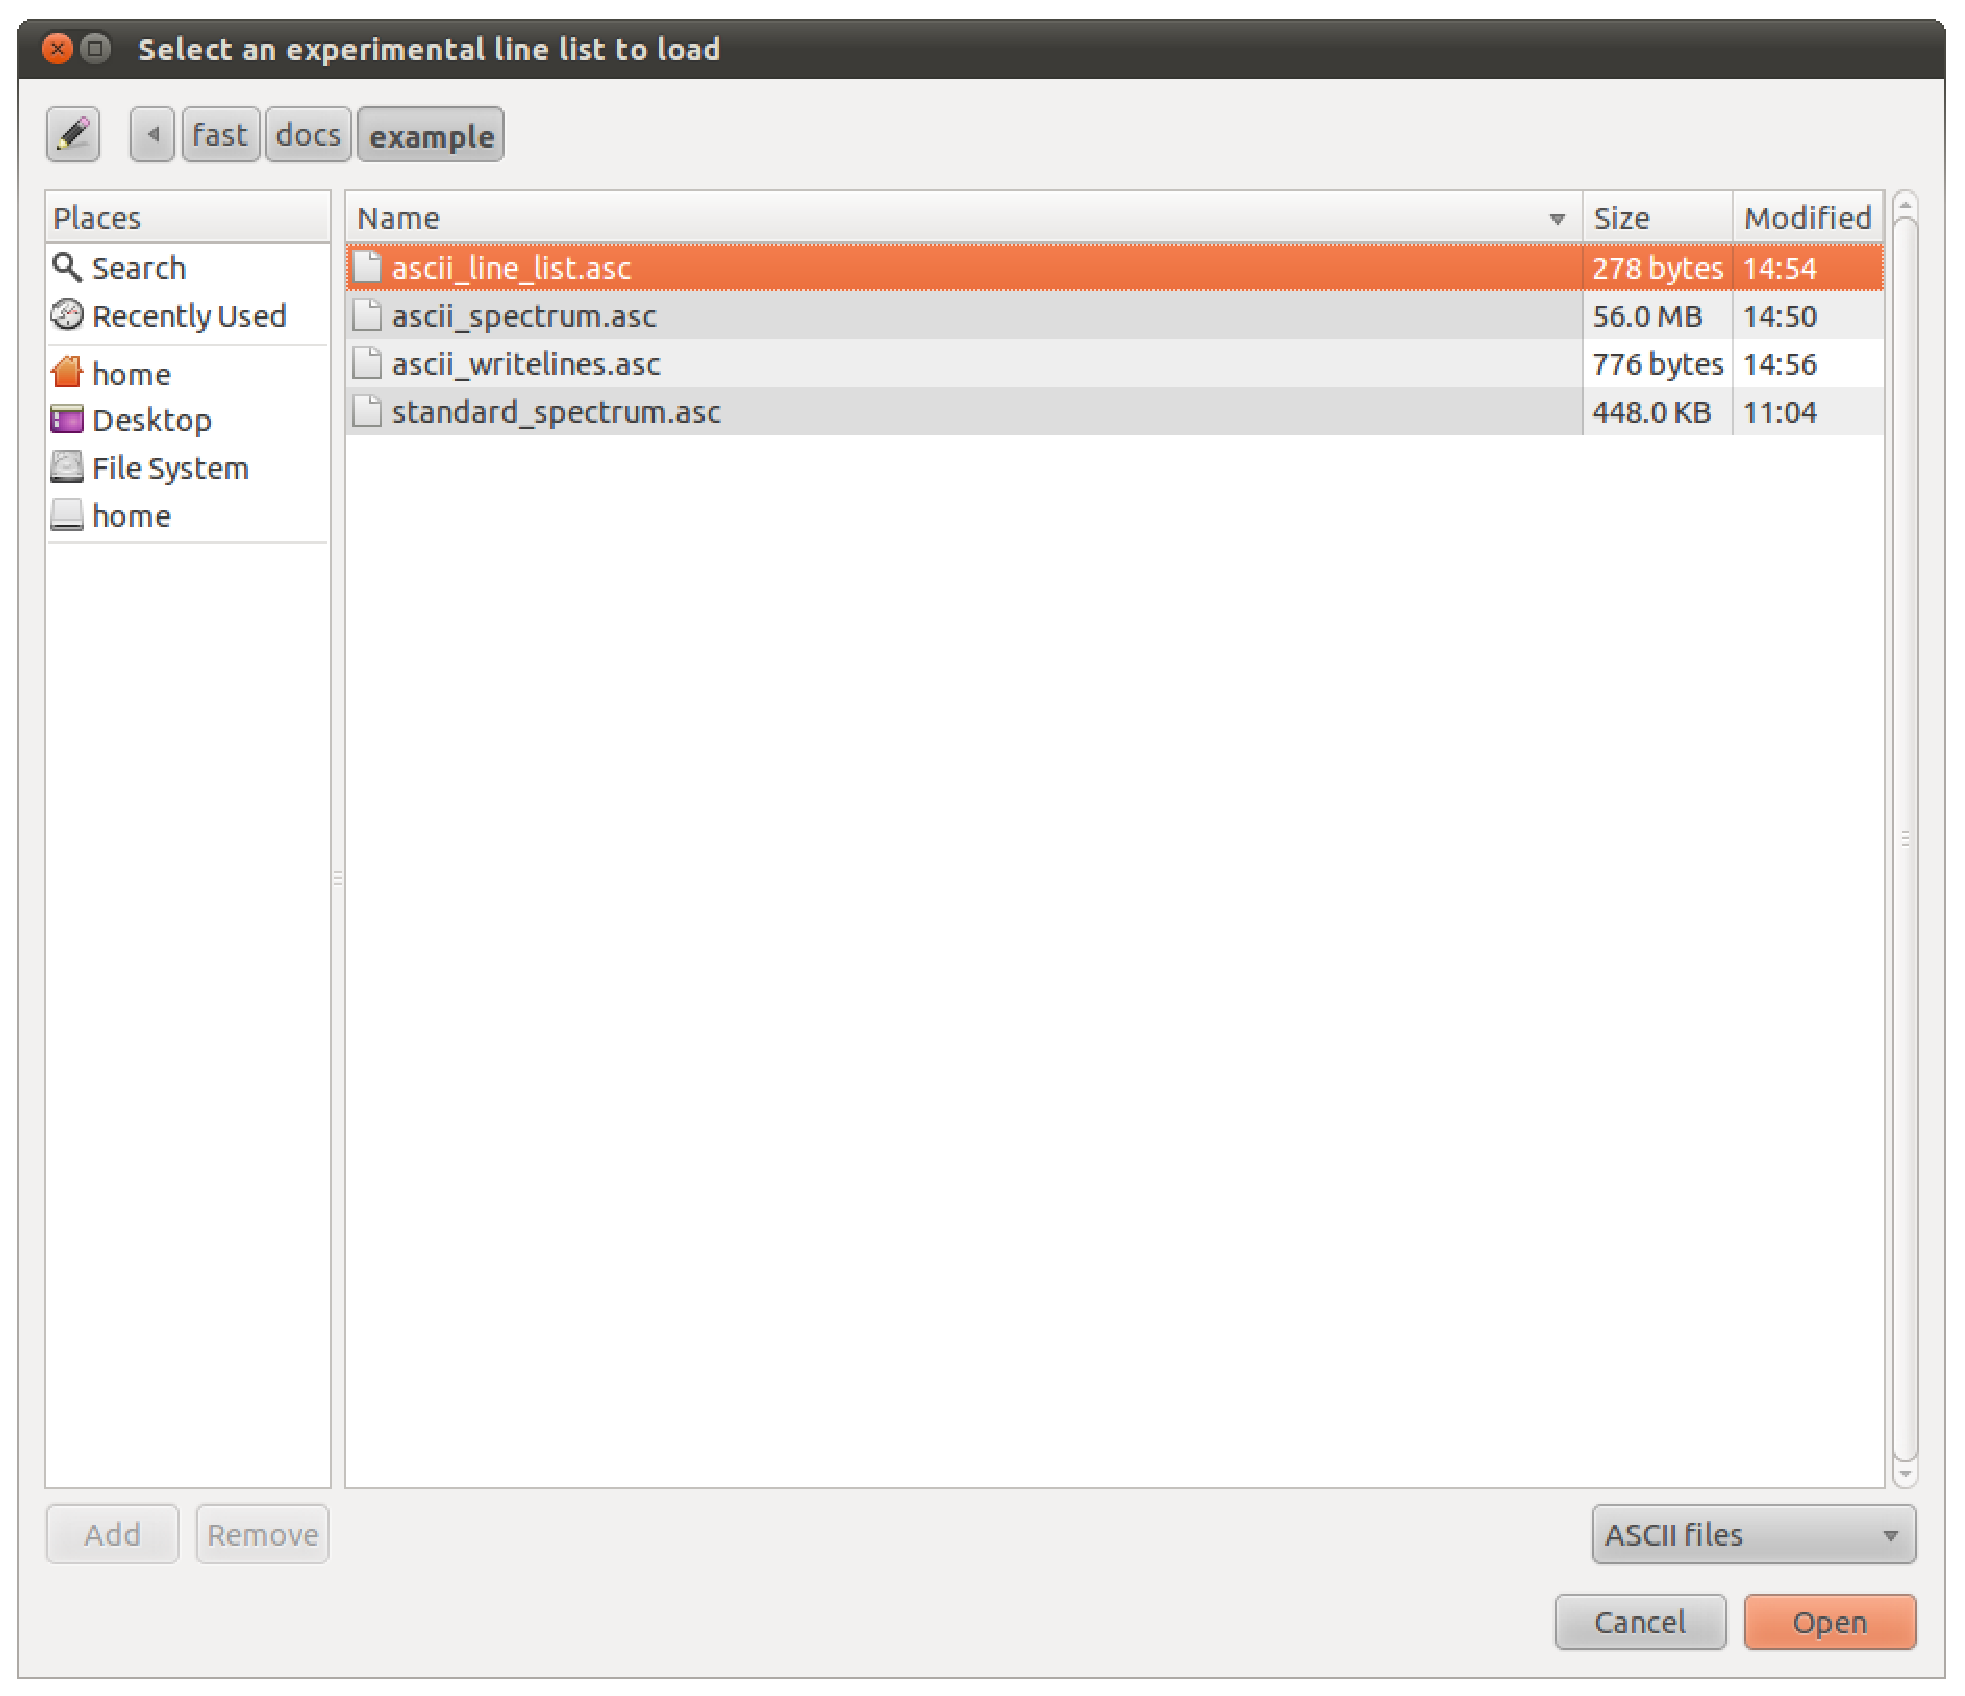
\includegraphics[width=140mm]{Tutorial5.eps}
\caption{Immediately afterwards, a second file open dialog will pop-up; this time requesting an experimental line list. Select `ascii\_line\_list.' from the list of files in the example folder, and click `Open'.}
\label{fig:tut5}
\end{figure}

\begin{figure}\centering
\includegraphics[width=140mm]{Tutorial6.eps}
\caption{These files will be added to the list of experimental data in pane (b), and the line profiles associated with the selected upper level plotted in pane (c). Select the ``Fitted Profiles" tab in pane (d) to view the line profile fit parameters. In pane (d) the line integrated intensities will be highlighted red as \fast is unable to intensity calibrate them.}
\label{fig:tut6}
\end{figure}

\begin{figure}\centering
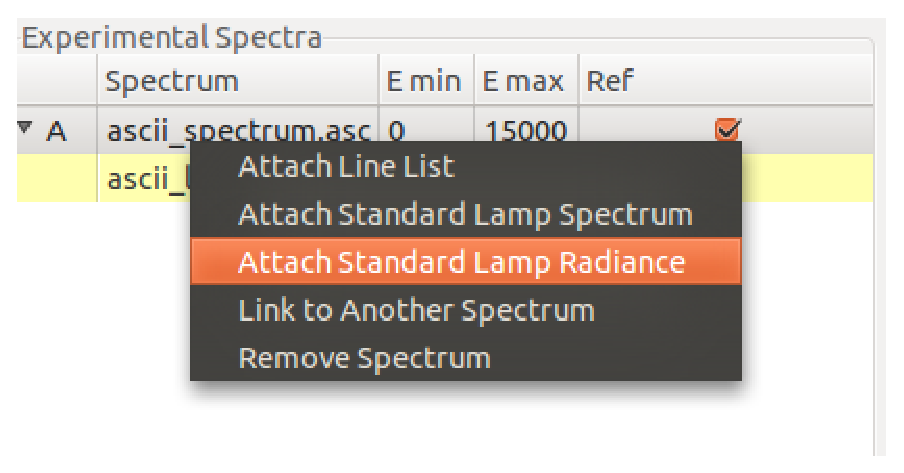
\includegraphics[scale=0.5]{Tutorial7.eps}
\caption{To allow \fast to intensity calibrate the experimental line profiles, first right click on `ascii\_spectrum.asc' in pane (b) and select "Attach Standard Lamp Radiance" from the pop-up menu that appears.}
\label{fig:tut7}
\end{figure}

\begin{figure}\centering
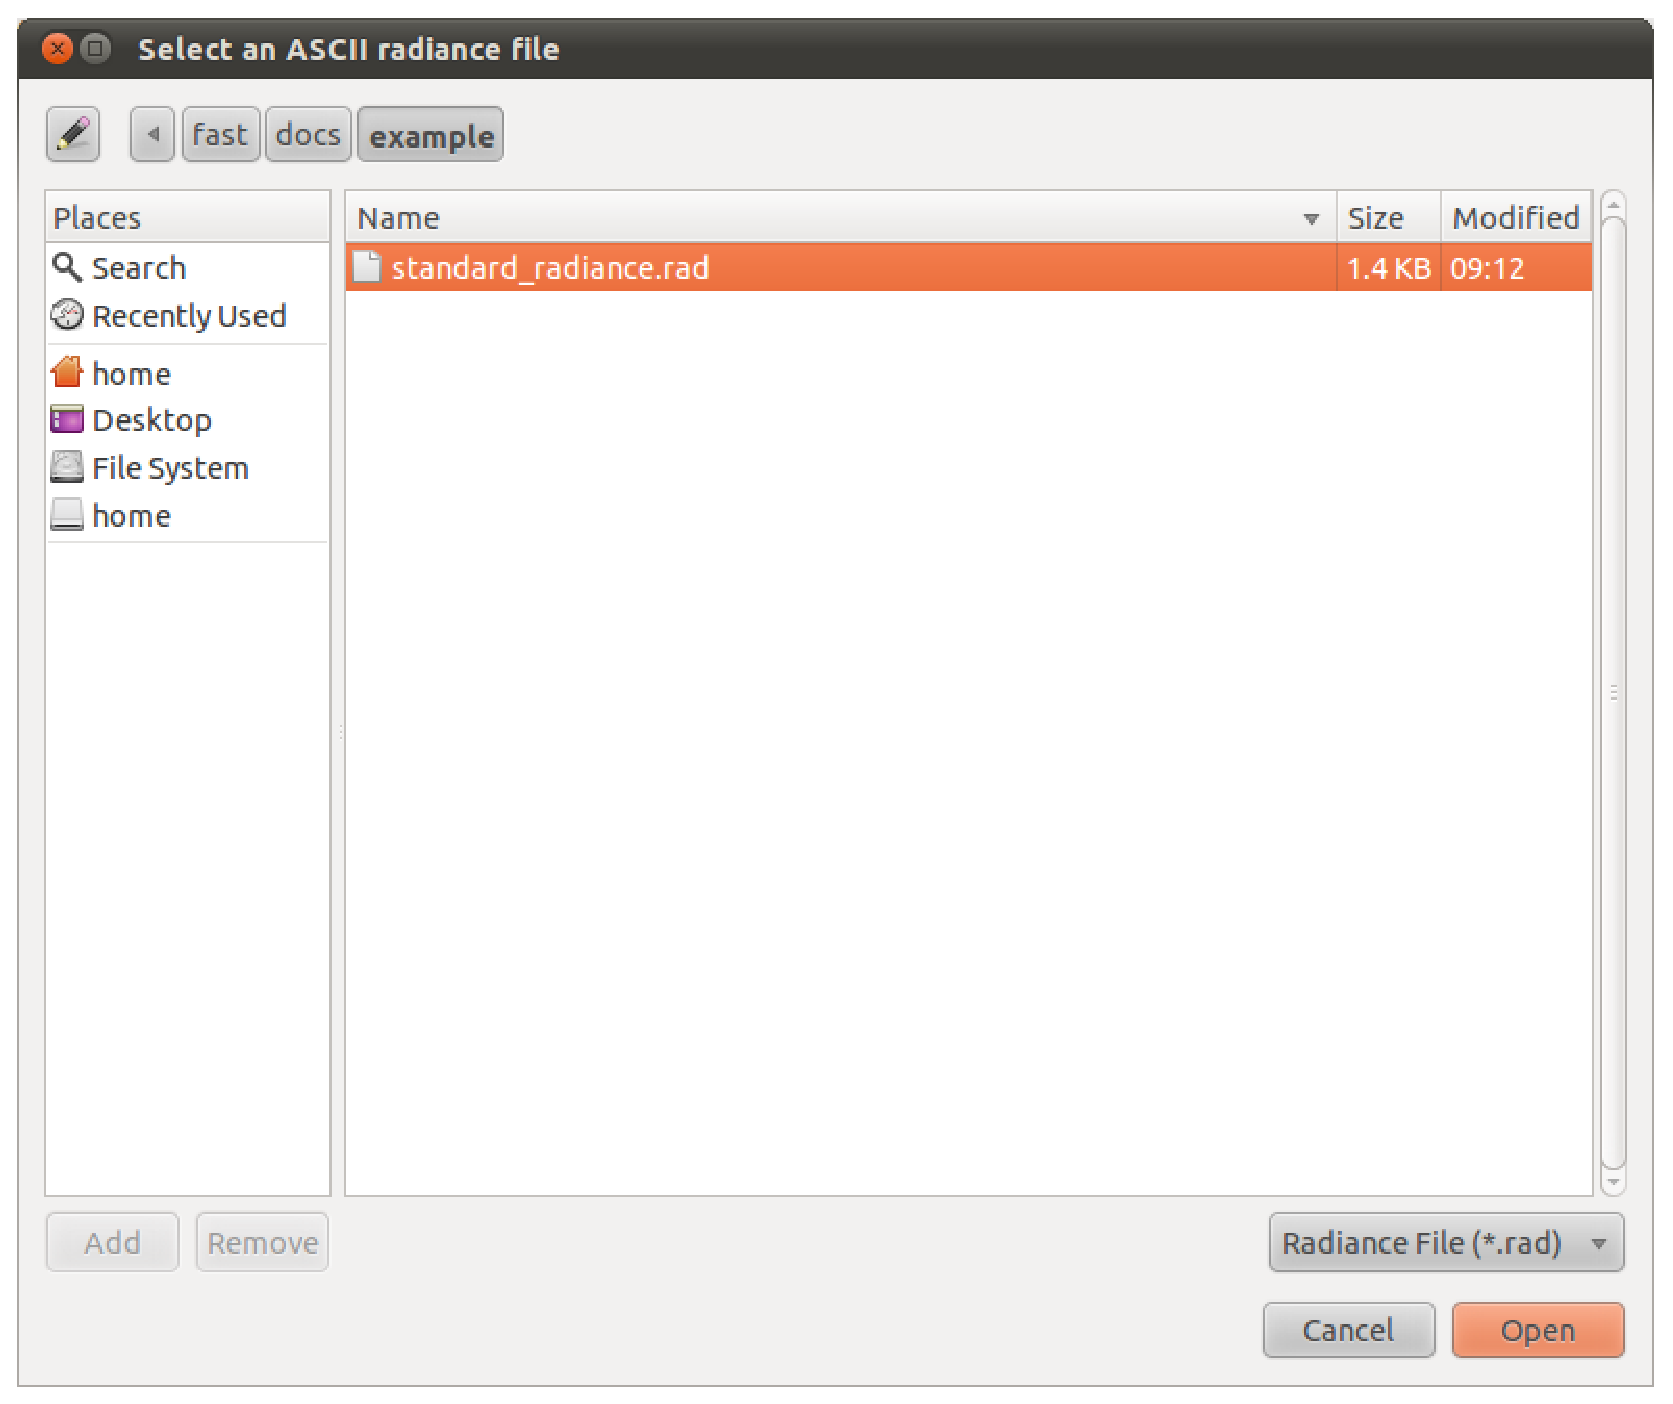
\includegraphics[scale=0.5]{Tutorial8.eps}
\caption{A file open dialog will pop-up asking for a standard lamp spectral radiance RAD file. Select `standard\_radiance.rad' from the list of files in the example folder, and click `Open'. This file is then attached to `ascii\_spectrum.asc' and listed in pane (b).}
\label{fig:tut8}
\end{figure}

\begin{figure}\centering
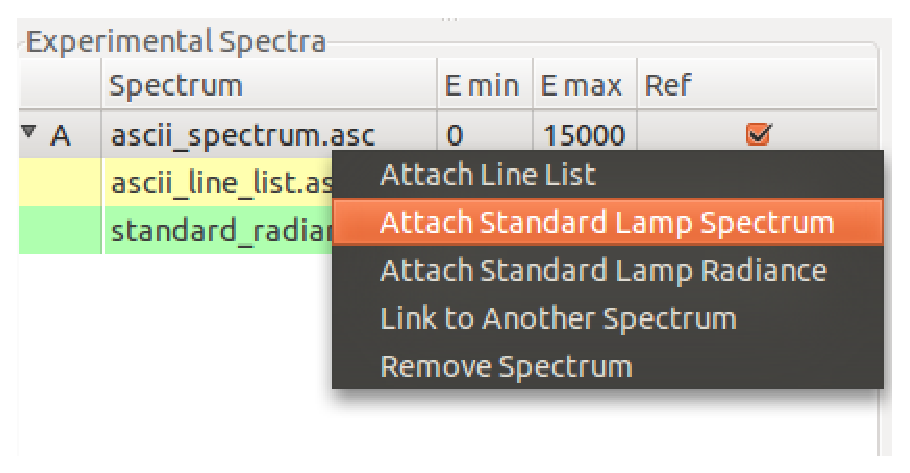
\includegraphics[scale=0.5]{Tutorial9.eps}
\caption{An observation of the same standard lamp is also required. Right click on 'ascii\_spectrum.asc' in pane (b) and select "Attach Standard Lamp Spectrum" from the pop-up menu that appears.}
\label{fig:tut9}
\end{figure}

\begin{figure}\centering
\includegraphics[width=140mm]{Tutorial10.eps}
\caption{Another file open dialog will pop-up, this time asking for a standard lamp spectrum. Select `standard\_spectrum.asc' from the list of files in the example folder, and click 'Open'. This file is then attached to `ascii\_spectrum.asc' and listed in pane (b).}
\label{fig:tut10}
\end{figure}

\begin{figure}\centering
\includegraphics[width=140mm]{Tutorial11.eps}
\caption{\fast now has all the information it requires for intensity calibration, so it automatically calculates the spectrometer response function from the standard lamp spectrum and spectral radiance data. This function is then used to correct the integrated intensities listed in pane (d). To indicate that this has been done successfully, the highlighting will change from red to green.}
\label{fig:tut11}
\end{figure}

\begin{figure}\centering
\includegraphics[width=140mm]{Tutorial12.eps}
\caption{To calculate atomic branching fractions for the loaded upper level, the transitions to be included in the sum over $i$ in equation \ref{eqn:bfexpt} must be selected. In the present case, all three experimentally observed line profiles must be included. Click on each one in turn. They will be highlighted blue once selected, and their predicted contribution to the total upper level BF added to the ``Complete" column in pane (a). Select the ``Branching Fractions" tab in pane (d) to view the BFs and associated data for each selected line.}
\label{fig:tut12}
\end{figure}

\begin{figure}\centering
\includegraphics[width=140mm]{Tutorial13.eps}
\caption{To obtain transition probabilities and oscillator strengths from the BFs, the upper level lifetime must be known. Select the ``Lifetimes" tab in pane (a) and insert the upper level lifetime where shown. The lifetime uncertainty must also be added, as shown. Once these numbers are entered, the transition probability and oscillator strength of each line is displayed in pane (d).}
\label{fig:tut13}
\end{figure}

\begin{figure}\centering
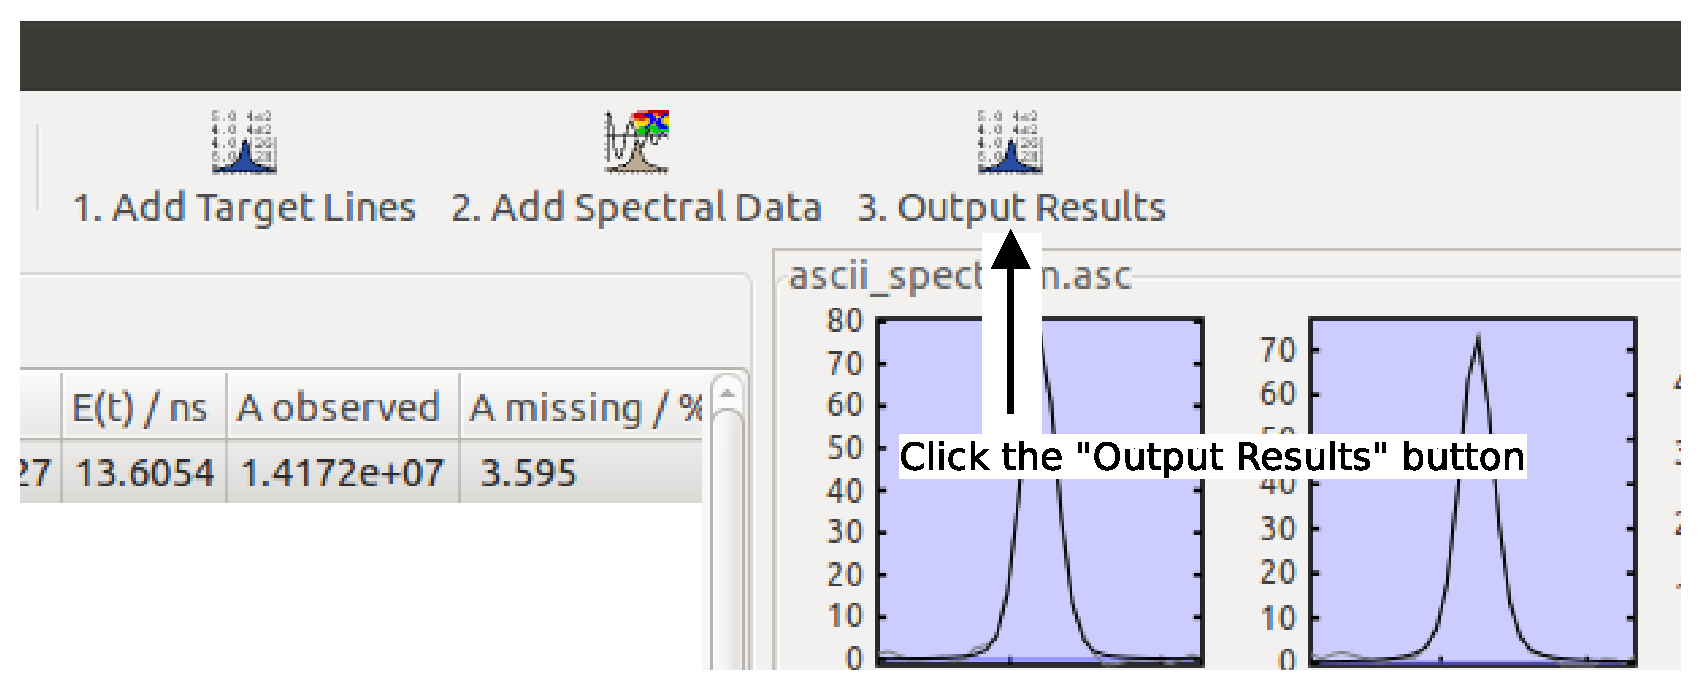
\includegraphics[scale=0.37]{Tutorial14.eps}
\caption{Once the branching fractions have been calculated to your satisfaction, they may be output in either Text/CSV or LaTeX format by clicking on the ``Output Results" button on the main toolbar.}
\label{fig:tut14}
\end{figure}

\begin{figure}\centering
\includegraphics[scale=0.45]{Tutorial15.eps}
\caption{A popup window will appear that allows the user to customise the output data. In the top-left of the window, one of three groups of fields may be selected - those relating to branching fractions, target lines, and fitted profiles. The fields belonging to selected groups are shown in the ``Available Fields" list. Select the fields that are to be output and add them to the list of "Selected Fields".}
\label{fig:tut15}
\end{figure}

\begin{figure}\centering
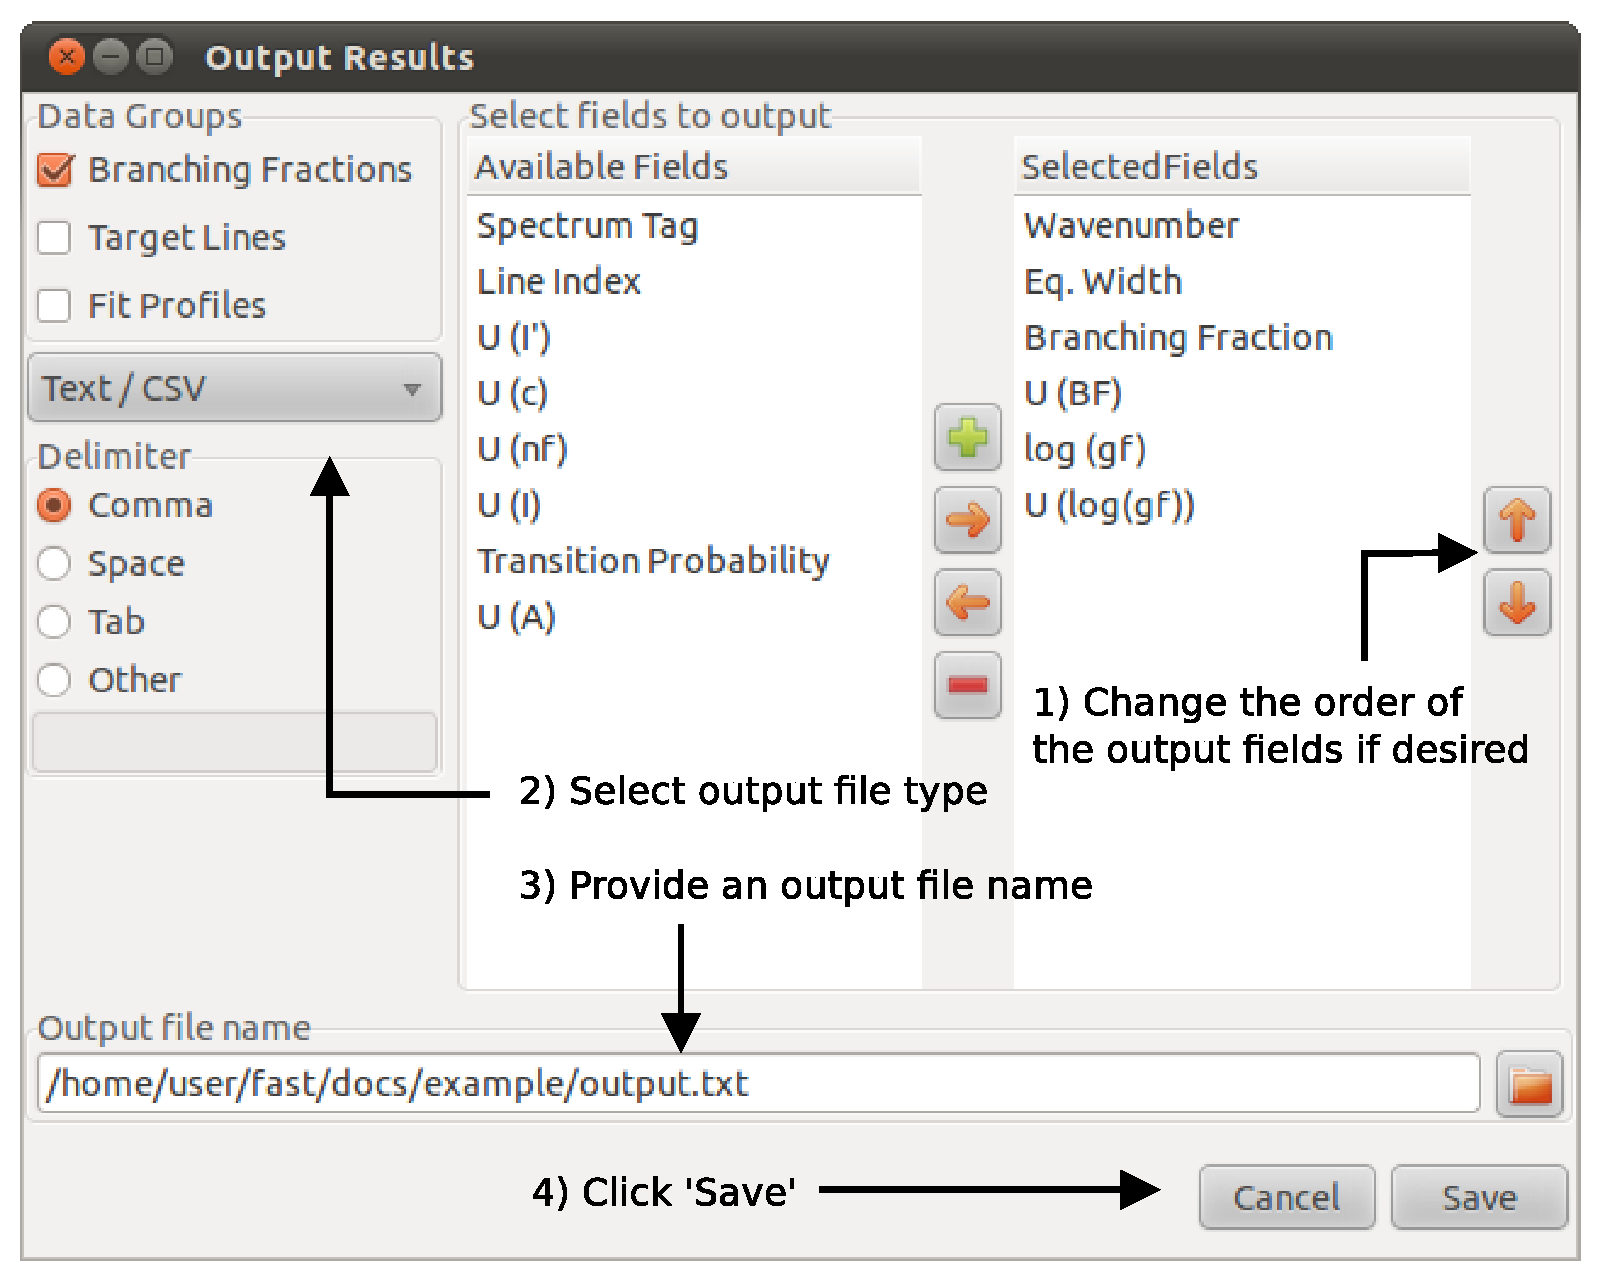
\includegraphics[scale=0.45]{Tutorial16.eps}
\caption{The order of the "Selected Fields" may be rearranged with the buttons on the right of the window. The output file type can be selected, as shown, on the left. Finally, specify an output file name and click ``Save".}
\label{fig:tut16}
\end{figure}

\end{document}
